% LaTeX mintafájl szakdolgozat és diplomamunkáknak az
% SZTE Informatikai Tanszekcsoportja által megkövetelt
% formai követelményeinek megvalósításához
% Modositva: 2011.04.28 Nemeth L. Zoltan
% A fájl használatához szükséges a magyar.ldf 2005/05/12 v1.5-ös vagy későbbi verziója
% ez letölthető a http://www.math.bme.hu/latex/ weblapról, a magyar nyelvű szedéshez
% Hasznos információk, linekek, LaTeX leirasok a www.latex.lap.hu weboldalon vannak.
%


\documentclass[12pt]{report}



\usepackage{ragged2e}
\usepackage{setspace}
%Magyar nyelvi támogatás (Babel 3.7 vagy későbbi kell!)
\def\magyarOptions{defaults=hu-min}
\usepackage[magyar]{babel}

%Az ékezetes betűk használatához:
\usepackage{t1enc}% ékezetes szavak automatikus elválasztásához
\usepackage[utf8]{inputenc}% ékezetes szavak beviteléhez

% A formai kovetelmenyekben megkövetelt Times betűtípus hasznalata:
\usepackage{times}

\usepackage{float}

%Az AMS csomagjai
\usepackage{amsmath}
\usepackage{amssymb}
\usepackage{amsthm}

%A fejléc láblécek kialakításához:
\usepackage{fancyhdr}

%Természetesen további csomagok is használhatók,
%például ábrák beillesztéséhez a graphix és a psfrag,
%ha nincs rájuk szükség természetesen kihagyhatók.
\usepackage{graphicx}
\usepackage{psfrag}

%a fákhoz
\usepackage[edges]{forest}

%Tételszerű környezetek definiálhatók, ezek most fejezetenkent egyutt szamozodnak, pl.
\newtheorem{tét}{Tétel}[chapter]
\newtheorem{defi}[tét]{Definíció}
\newtheorem{lemma}[tét]{Lemma}
\newtheorem{áll}[tét]{Állítás}
\newtheorem{köv}[tét]{Következmény}

%Ha a megjegyzések és a példak szövegét nem akarjuk dőlten szedni, akkor
%az alábbi parancs után kell őket definiální:
\theoremstyle{definition}
\newtheorem{megj}[tét]{Megjegyzés}
\newtheorem{pld}[tét]{Példa}

%Margók:
\hoffset -1in
\voffset -1in
\oddsidemargin 35mm
\textwidth 150mm
\topmargin 15mm
\headheight 10mm
\headsep 5mm
\textheight 237mm

%\usepackage{titlesec}
%\titlespacing*{\chapter}
%{0pt}{12pt}{12pt}

\usepackage{titlesec}
\begin{document}

\titleformat{\chapter}[display]   
{\normalfont\huge\bfseries}{\thechapter .\ \chaptertitlename}{20pt}{\Huge}   
\titlespacing*{\chapter}{0pt}{-40pt}{40pt}
\onehalfspacing
%A FEJEZETEK KEZDŐOLDALAINAK FEJ ES LÁBLÉCE:
%a plain oldalstílust kell átdefiniálni, hogy ott ne legyen fejléc:
\fancypagestyle{plain}{%
%ez mindent töröl:
\fancyhf{}
% a láblécbe jobboldalra kerüljön az oldalszám:
\fancyfoot[R]{\thepage}
%elválasztó vonal sem kell:
\renewcommand{\headrulewidth}{0pt}
}

%A TÖBBI OLDAL FEJ ÉS LÁBLÉCE:
\pagestyle{fancy}
\fancyhf{}
\fancyhead[L]{Automataelméleti feladatok generálása}
\fancyfoot[R]{\thepage}

\thispagestyle{empty}
\begin{center}
{\fontsize{18}{21}\selectfont\bf Szegedi Tudományegyetem}

\vspace{0.5cm}

{\fontsize{18}{21}\selectfont\bf Informatikai Intézet}

\vspace{7cm}

{\fontsize{24}{28}\selectfont\bf SZAKDOLGOZAT}

\vspace{10cm}

{\fontsize{22}{24}\selectfont\bf Bencsik Dávid}

\vspace{0.5cm}

{\fontsize{18}{21}\selectfont\bf 2018}
\end{center}
\newpage
%A címoldalra se fej- se lábléc nem kell:
\thispagestyle{empty}

\begin{center}
\vspace*{1cm}
{\Large\bf Szegedi Tudományegyetem}

\vspace{0.5cm}

{\Large\bf Informatikai Intézet}

\vspace*{3.8cm}


{\LARGE\bf Automataelméleti feladatok generálása}


\vspace*{3.6cm}

{\Large Szakdolgozat}
% vagy {\Large Szakdolgozat}

\vspace*{4cm}

%Értelemszerűen megváltoztatandó:
{\large
\begin{tabular}{c@{\hspace{4cm}}c}
\emph{Készítette:}     &\emph{Témavezető:}\\
\bf{Bencsik Dávid}  &\bf{Dr. Fülöp Zoltán}\\
programtervező informatikus BSc     &egyetemi tanár\\
szakos hallgató&
\end{tabular}
}

\vspace*{2.3cm}

{\Large
Szeged
\\
\vspace{2mm}
2018
}
\end{center}

%A \chapter* parancs nem ad a fejezetnek sorszámot
\chapter*{Feladatkiírás}
%A tartalomjegyzékben mégis szerepeltetni kell, mint szakasz(section) szerepeljen:
\addcontentsline{toc}{section}{Feladatkiírás}

A hallgató feladata a reguláris nyelvek tulajdonságainak és a véges automata
konstrukcióknak (egyesítést, metszetet, iteráltat felismerő automata, minimalizálás) az áttekintése
és ezeknek egységes módon történő leírása. Gyakorlati részként a hallgató készítsen olyan
programot, amely automataelméleti feladatokat generál, képes megoldásokat fogadni és
kiértékelni.

\chapter*{Tartalmi összefoglaló}
\addcontentsline{toc}{section}{Tartalmi összefoglaló}

A szakdolgozatomban egy feladatgeneráló programot írok C++ nyelven. A célom végeredményben egy olyan módszer kidolgozása, amellyel tetszőleges témájú feladatokat lehet véletlenszerűen generálni az egyes diákok igényeihez igazítva. Ez hasznos lehet tanároknak a munkájuk megkönnyítéséhez, illetve e-learning rendszerek alapját is képezheti. Ez az általános program azonban igen összetett, ezért a rendelkezésre álló időben egyenlőre egy olyan generátort valósítok meg, amely egy fix témában ad feladatokat.

Ez a téma a véges automatákkal kapcsolatos feladat. Ilyen feladat például:\\

\textit{"Adj meg olyan $\{$a,b$\}$ abc-jű automatát amely a következőt ismeri fel: szó, amelyben $|W|_a$ 3-mal osztható!"}.
\\

Választásom azért esett a véges automatákra, mert közel állnak a számítástudományi alapproblémákhoz, így a véletlen-generáláshoz is.

A szakdolgozat bemutatja a fentebb felvázolt témát, ismerteti a feladatokat, a generálási módszert, az ehhez szükséges algoritmusokat, továbbá ezek elméleti, gyakorlati jellegű kérdéseit boncolgatja.

Szó lesz továbbá a feladatgeneráló felhasználásának lehetőségeiről, ezek hatékonyságáról, hasznosságáról.
\\

Kulcsszavak: véges automata, feladatgenerátor, procedurális generálás, e-learning

\chapter*{Bevezetés}
\addcontentsline{toc}{section}{Bevezetés}
Napjainkban a technológia és a népesség robbanásával egyre homályosabbá válik az ember, a gép és az intelligencia viszonya. Ahhoz, hogy az oktatás ki tudja elégíteni a munkaerőpiac folyamatosan változó igényeit és hogy a gépesítés miatt munkájukat veszítő emberek tovább tudják magukat képezni, minden eszközre szükség van.\\

Ilyen eszközök a tanintézményekben az oktatók munkáját segítő rendszerek, vagy például az e-learning rendszerek, amelyekkel egy weboldalról is tanulhatnak az arra vágyó emberek.
Ezen rendszereknek fontos funkciója, hogy azokon a tanulók feladatokat tudjanak kapni, és a megoldásuk helyességét is ellenőrizni tudja a rendszer. Ezen feladatokat kézzel is felvihetik a rendszerbe az oktatók, de sokat könnyít a munkájukon, hogy ha a program is képes magától feladatokat adni, vagy legalább a felvitt feladatokat kis mértékben variálni, hogy ne mindenki ugyanazt kapja. A szakdolgozatomban egy ilyen automatikus feladat-generáló rendszert ismertetek és implementálok C++ nyelven. A feladatok témája a véges automaták.

Eredetileg szerettem volna egy teljes e-learning rendszert kialakítani, nem csupán a feladat-generátort, de erre sajnos nem jutott időm.\\

Egy ilyen generáló program felépítése nagyon egyszerű is lehet, ha kompromisszumokat vállalunk, de ha szeretnénk a program működését olyan jóra megcsinálni, mint ahogy azt álmainkban elképzelnénk, akkor nagyon gyorsan komoly számítástudományi problémákba ütközünk. Ezen problémák egy részét a szakdolgozatban jellemzem és megmutatom a megoldásukat, vagy olyan módszereket, amelyek bizonyos mértékben megoldják azokat. Sok probléma azonban meghaladja szakmai képességeimet, ezekről is szót ejtek.\\

Azért vágtam neki ennek a témának, mert szerintem nagyon érdekes és úgy gondolom, hogy közvetett módon a területnek társadalmi hasznossága is van. Korábban is foglalkoztam hasonló jellegű problémákkal, de az egyetemi tanulmányaim és a szakdolgozat készítése során sokat nőtt a tudásom, amellyel később talán nehezebb feladatokat is meg tudok majd oldani, esetleg kézzel fogható eredményt produkálni. Ilyen eredmény lenne a szakdolgozatban vázolt működés kiterjesztése tetszőleges témákra és egy e-learning rendszer kifejlesztése ami használható és hasznos.

%A tartalomjegyzék:
\tableofcontents

\chapter{Véges automaták}
Ahhoz, hogy véges automatás feladatokról beszélhessünk, először meg kell mutatnom mik azok a véges automaták. Ehhez azonban egy sor alapfogalmat kell megismernünk. Ezek a fogalmak fontosak lesznek majd a generálásnál is.

A véges automatákkal kapcsolatos fogalmakat, algoritmusokat Fülöp Zoltán Formális nyelvek és szintaktikus elemzésük című könyvéből \cite{Fulop} tanultam meg.

\section{Alapfogalmak}
\subsection{Abc}
Szimbólumoknak egy tetszőleges véges, nem üres halmaza. $\Sigma$ (Szigma)-val jelöljük.

\begin{center}
Pl.: $\Sigma=\{a,b,c,d\}$
\end{center}
\subsection{Abc feletti szavak}
$\Sigma$ abc feletti szavak $a_1...a_k$ sorozat, ahol $k\geq0$ és  $a_1...a_k\in\Sigma$.\\
Ha $k=0$, azt üres szónak hívjuk, jele: $\epsilon$ (epszilon).
\begin{center}
$\Sigma=\{a,b\}$ abc-nek pl. szavai: $\epsilon,a,b,aa,ab,ba,bb,aaa...$(és még végtelen sok)
\end{center}
$\Sigma$ feletti összes szó halmazát $\Sigma^*$-al jelöljük:
\begin{center}
$\Sigma^* = \{a_1...a_k | k\geq0, a_1,...,a_k\in\Sigma \}$
\end{center}
\subsection{Szavakkal kapcsolatos jelölések}
$a^n$ = $n$ darab egymást követő $a$ betű (Pl. $a^5$ = $aaaaa$)\\
$a^*$ = akárhány darab egymást követő $a$ betű (akár 0 is)\\
$a^+$ = 1 vagy annál több darab egymást követő $a$ betű

Amikor azt írjuk $ab$, akkor nyilvánvaló, hogy egy $a$ betűt követ egy $b$. Ez pontosan így van a összetett jelöléseknél is. Pl.: $a^nb^n$ = n darab $a$ betűt követ $n$ darab $b$ betű, tehát $a^3b^3$ = $aaabbb$. Ezt a betűk, vagy szavak konkatenációjának nevezzük.

Továbbá pár logikai jelölés:\\
$A\land B$ : logikai és\\
$A\lor B$ : logikai vagy\\
$\neg A$ : logikai negálás\\
Tehát a következő mondatot: \textit{"Nem esik az eső és fúj a szél."} a logika nyelvén így is írhatjuk : \textit{"$\neg$(Esik az eső) $\land$ (Fúj a szél)"}\\
$\{...\}$ : halmaz definíció\\
$a\in\Sigma$ : $a$ eleme $\Sigma$ halmaznak\\
$a\notin\Sigma$ : $a$ nem eleme $\Sigma$ halmaznak
\subsection{Nyelv}
\textbf{Definíció.} $\Sigma^*$ tetszőleges részhalmazát $\Sigma$ feletti nyelvnek nevezzük.\\

Általában $L$-el jelöljük. $aba\in L$ azt jelöli, hogy $aba$ szó az $L$ nyelvnek eleme.\\

Példák $\Sigma=\{a,b\}$ feletti nyelvekre:

\begingroup
\leftskip1.5em
\rightskip\leftskip
\noindent
\hangindent=2em
\hangafter=1
$L = \{aaa,bab,bbbba,a,\epsilon\}$ : Ez egy véges nyelv, amelyet egyszerűen az elemei felsorolásával adtunk meg. A véges azt jelenti, hogy véges sok eleme van.

\noindent
\hangindent=2em
\hangafter=1
$L = \{a^nb^n|n>2\}$ : Ezt a nyelvet formulával adtuk meg. A formula jelentése: a szóban $n$ darab $a$ betűt $n$ darab $b$ követ, és $n$ kettőnél nagyobb. Például $aaabbb\in L$, de $abbb\notin L$. Ha belegondolunk, ez egy végtelen nyelv, hiszen végtelen sok ilyen szó van.Az efféle jelölésben általánosan a $|$ jel bal oldalán valamilyen paraméterezett alakot adunk a nyelvben levő szavaknak, és a jobb oldalon megkötjük a paramétereket.

\noindent
\hangindent=2em
\hangafter=1
$L = \{w \in \Sigma^*|$\textit{w-ben minden a után áll egy b}$\}$ : Ebben a formulás jelölésben a bal oldalon csupán annyit írtunk, hogy $w$ egy tetszőleges $\Sigma$ feletti szó(tehát itt még bármi lehet), és a jobb oldalon egy magyar mondattal adunk megkötést a szóra. Például $bbabbbab\in L$, de $aab\notin L$, továbbá $\epsilon\in L$, hiszen az üres szóra is igaz a megkötés. Ez szintén végtelen nyelv.
\\

\endgroup
Tehát elég sokféleképpen adhatóak meg nyelvek(nem csak ez a 3 fajta).

Fontos itt megjegyezni, hogy a nyelv szó hétköznapi értelme eltér a fönti definíciótól. A magyar nyelvet nem szokás egyszerűen a szótárban levő lehetséges szavakkal azonosítani. El kell tehát vonatkoztatnunk a nyelv hétköznapi jelentésétől. A fentebb felvázolt formális definíció számunkra hasznosabb lesz és számítástudományokban ezt használjuk.

\subsection{Műveletek nyelvekkel}
Vegyük az $L_1,L_2,L_3 \subseteq \Sigma^*$ nyelveket. A legfontosabb műveletek a következők:

\begin{itemize}
\item $L_1 \cup L_2$ a két nyelv uniója, ez, mivel a nyelvek halmazként is kezelhetőek, azt jelenti, hogy az uniójukban minden szó benne lesz, amelyik legalább az egyikben benne van.
\item $L_1 \cap L_2$ a két nyelv metszete.
\item $L_1 - L_2$ a két nyelv különbsége.
\item $\overline{L_1} = \Sigma^* - L_1$ az $L_1$ komplementere, tehát minden szó, ami az $L_1$-hez tartozó abc-ből előállhat, de $L_1$-ben nincs benne.
\item $L_1L_2$ a két nyelv konkatenációja. Ez azt jelenti, hogy vesszük $L_1$ összes szavát, illetve $L_2$ összes szavát, és egymás után tesszük őket minden lehetséges kombinációban, például $\{ab,aa\}\{a,bb\} = \{aba,aaa,abbb,aabb\}$.
\item $L_1^n$ az $L_1$ $n$-dik hatványa, ez azt jelenti, hogy a nyelvet $n$-szer saját magához konkatenáljuk.
\item $L_1^*$ az $L_1$ Kleene-starja, vagy más néven iteráltja, ez azt jelenti, hogy $L_1$-et tetszőlegesen sokszor (akár 0-szor) maga után konkatenáljuk.
\item $L_1^+$ ez pedig ugyanaz, mint az $L_1^*$, csak a 0-szor konkatenálást kizárjuk.
\end{itemize}

\subsection{Automata}
Az automaták absztrakt számítógép-modellek, amelyek feladata, hogy megállapítsák a bemenetén kapott értékről, hogy az bizonyos feltételeknek megfelel, vagy sem. Ha megfelel, az automata elfogadja(felismeri), ha nem, akkor elutasítja(nem ismeri fel).

Egy rendes számítógép ennél bonyolultabb dolgokat is csinál, például adatokat tárol a merevlemezen stb., de számunkra elméleti szempontból elég azt vizsgálni, hogy egy bemenetet elfogad-e vagy sem.

Ez azért is előnyös, mert így az automaták közvetlen kapcsolatba kerülnek a halmazokkal, ugyanis azt mondhatjuk, hogy az automata által elfogadott értékek egy halmazba tartoznak, így az automata egy halmazt is kijelöl. Ilyen halmazok a nyelvek is, ezért az automata bemenetét \textit{szó}-nak szokás hívni, az automatáról pedig azt mondjuk, hogy az felismeri, hogy a bemenetként kapott szó eleme-e az adott nyelvnek.

Automatából sokféle van, egyik fajtájuk a véges automata, amellyel a szakdolgozatban foglalkozni fogok. Sokszor a véges automatákat csak simán automatáknak hívom, ez egy rövidítés, remélhetőleg nem túl zavaró.

\section{Véges automata}

\begin{figure}[H]
\centering
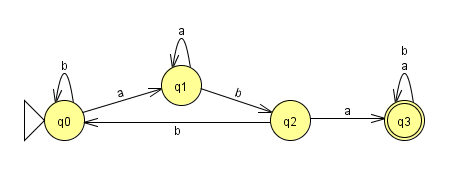
\includegraphics[scale=1]{abaresze.png}
\caption{\label{aut} Példa véges automatára}
\end{figure}

Az ábrán egy véges automata látható, ez az automata ha bemenetként kap egy szót, akkor felismeri, hogy a szó tartalmaz-e $aba$-t. Például ha a bemenetén kap egy $aaab$ szót, akkor azt végigolvassa, majd megállapítja, hogy ez nem tartalmazza az $aba$ részszót. Tehát a gép az $aaab$ szót nem fogadja el (elutasítja).

De ha például bemenetként $babaa$-t kap, azt végigolvasva azt el fogja fogadni.

A következőképp működik: A nyíllal jelölt $q0$ kezdőállapotból indul. Ekkor megnézi a szó első betűjét. Ha $a$, akkor továbblép $q1$-be, ha $b$ akkor pedig egy helyben marad.

A nyilakból minden állapotnál látható, hogyha az adott állapotba adott betűt kap, akkor merre megy tovább.

Amennyiben a szót végigolvasta, megáll. Ha kétszer karikázott állapotban áll meg (végállapot), akkor a szót elfogadja(felismeri), különben nem(elutasítja).

Több ilyen végállapot is lehet, de kezdőállapot csak egy. Továbbá minden állapotból kell, hogy menjen nyíl minden $abc$-beli betűre (az $abc$ itt $\Sigma = \{a,b\}$).

Formálisan a következőkkel tudunk egyértelműen definiálni egy automatát:\\
$M = (Q, \Sigma, \delta, q0, F)$-t véges automatának nevezzük, ahol:
\begin{enumerate}
\item $Q$ egy nem üres, véges halmaz, az állapotok halmaza,
\item $\Sigma$ egy $abc$, az input $abc$,
\item $q0 \in Q$ a kezdő állapot,
\item $F \in Q$ a végállapotok halmaza,
\item $\delta : Q \times \Sigma \to Q$ egy leképezés, az átmenetfüggvény.
\end{enumerate}

\subsection{Véges automatás feladatok}
A szakdolgozatban tárgyalt és megvalósított feladatgeneráló véges automatás feladatokat generál.

Ilyen például a következő:

\textit{"Adj meg olyan $\{a,b\}$ abc-jű automatát amely a következőt ismeri fel: szó, amelyben minden a-t b követ!"}

A hallgató feladata, hogy fölírjon egy automatát, amely pontosan azokat a szavakat fogadja el, amelyekben minden $a$-t $b$ követ.

A beküldött megoldást pedig a rendszer értékeli, hogy helyes-e.

\subsection{Véges automatával felismerhető nyelvek}
Fölmerülhet a kérdés, hogy egy ilyen kezdetleges gép mennyire tud összetett tulajdonságokat fölismerni a szavakkal kapcsolatosan. A válasz az, hogy meglepően sok mindent, de van olyan amit nem, például:

\textit{"Adj meg olyan $\{a,b\}$ abc-jű automatát amely a következőt ismeri fel: az a-k száma megegyezik a b-k számával"}

Nincs olyan véges automata, amely ezt felismerné. Röviden azért, mert ehhez meg kellene számolnia az $a$-k számát a szóban, de ebből tetszőleges sok lehet, az állapotaink száma pedig fix, véges. Ezért ilyen feladatot nem is kaphat a hallgató.

Általánosan elmondható, hogy a véges automaták pontosan a reguláris nyelveket ismerik fel. A reguláris nyelvek igen egyszerű nyelvek, melyek előállíthatóak szavak konkatenációjával, uniójával és iterációjával. Számos tulajdonsága van ezeknek a nyelveknek, de ebbe részletesebben nem megyek bele.

A lényeg, hogy a feladatok mind reguláris nyelveket határoznak meg, mert pontosan ezek ismerhetők fel véges automatákkal.

\section{Feladat ellenőrzés}
Ahhoz, hogy kiértékeljük a hallgató által beküldött feladatot, összehasonlítjuk egy megoldással ami biztosan jó (\textit{etalon}). Ezt a megoldást a generálási folyamat a feladat szövegével együtt előállítja. Ez azért nem triviális, mert egy nyelvhez több véges automata is van, amely azt felismeri. Tehát többféle helyes megoldás létezik.

A feladatunk a két véges automata (a beküldött és az etalon) összehasonlítása. Erre több módszer is létezik, íme pár.

\subsection*{Minimalizálással}
Tudjuk azt, hogy ha két véges automata ugyanazt a nyelvet ismeri fel, akkor a minimalizáltjuk megegyezik. Illetve nem teljesen, mert ugyan a minimalizált automaták szerkezetükre teljesen megegyeznek, az állapotaik címkéi lehetnek mások.

Ha egy automata állapot-címkéinek átszámozásával megkapjuk a másikat, akkor a két automata izomorf.

A módszer tehát a következő: Minimalizáljuk mind a két automatát, majd megnézzük, hogy izomorfak-e.

Azt, hogy mi az a minimalizálás, a szakdolgozat egy későbbi fejezetében (1.4.2) ismertetem.

\subsection*{Halmazelmélettel}
A két nyelvet, $L_1$-et és $L_2$-t halmazként tekintve pont úgy, mint bármely más halmazra teljesül az, hogy ha ekvivalensek, akkor, és csak akkor ($L_1-L_2$) üres és ($L_2-L_1$) üres.

Ezeket a halmazelméleti műveleteket pedig automatákkal is el tudjuk végezni. Ez a módszer nagyon egyszerű és nagyon lassú is, mert a halmazműveletek a direkt szorzat miatt négyzetes idejűek.

Ugyanakkor kevés állapotra teljesen jól működik és csak pár sor leírni, ezért a programban ezt a módszert használom.

Az algoritmus implementációja a forráskódban a \textbf{DFA::equals(DFA other)} metódus.

\subsection*{Hopcroft és Karp}
A leggyorsabb algoritmust Hopcroft és Karp\cite{Hopcroft and Karp} írták, ami lineáris. Lényegében annyit csinál, hogy a két automata állapotait a kezdő állapotból minden átmenetre párhuzamosan bejárja, és ha egy ilyen állapotpárban az egyik automata elfogad, a másik pedig nem, akkor nem ekvivalensek. Ha pedig bejárta az átmeneteit mind a kettőnek és ilyet nem talált, akkor ekvivalensek.

\section{Algoritmusok}
Itt pár lényeges algoritmust írok le véges automaták konstrukciójához. Ezeket és még többet, a programban le is implementáltam.

\subsection{Direkt szorzat}
Fentebb már beszéltem arról, hogy a logikai műveletek halmazelméleti műveletekké alakíthatóak (pl. \textit{és $\rightarrow$ metszet}) és hogy ezek a műveletek elvégezhetőek konstrukciókkal automatákon is. Az összes halmazelméleti művelet hasonlóképp történik, mindegyiknek az alapja a direkt szorzat. A konstrukciót egy példán keresztül mutatom be.
\begin{figure}[H]
\centering
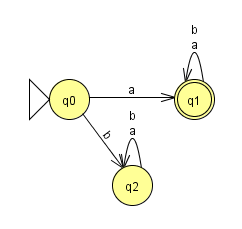
\includegraphics[scale=1]{direkt_a_val_kezd.png}
\caption{\label{direkt-egy} Automata, mely felismeri, ha a szó $a$-val kezdődik}
\end{figure}

\begin{figure}[H]
\centering
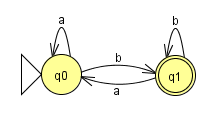
\includegraphics[scale=1]{direkt_b_re_vegzodik.png}
\caption{\label{direkt-ketto} Automata, mely felismeri, ha a szó $b$-re végződik}
\end{figure}

A \ref{direkt-egy} és \ref{direkt-ketto} ábrákon látható automatáknak az és kapcsolatba helyezése egy olyan automata, amely felismeri, ha a szó $a$-val kezdődik és $b$-re végződik. Ezt az automatát elő tudjuk állítani egy algoritmussal.

Ehhez azt kell belátnunk, hogy az és kapcsolatuk az pont az, mintha a két automatát egyszerre futtatnánk, és figyelemmel kísérnénk, hogy közben az egyik és a másik automata épp milyen állapotot vesz fel. A direkt szorzat konstrukció pont ezt teszi.

Vázlatosan az algoritmus:
\begin{enumerate}
            \item Felírjuk az összes lehetséges állapotpárt (pl $(q0;q2)$) és felvesszük őket, mint állapotokat az új automatába.
            \item Az így kapott állapotokból behúzzuk minden betűre az átmeneteket. Például, ha az egyik automata $q0$-ból $a$ betű hatására $q2$-be lépett, míg a másik automata $q2$-ből $a$ betű hatására $q3$-ba lépett, akkor az új automata $(q0;q2)$-ből $a$ betű hatására $(q2;q3)$-ba lép.
            \item A kezdő állapotunk az a pár lesz, amelyben a két automata kezdőállapotai vannak  (pl. itt $(q0;q0)$).
\end{enumerate}

\begin{figure}[H]
\centering
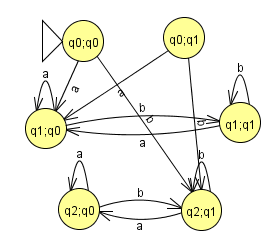
\includegraphics[scale=1]{direkt_a-val_kezdodik_szorzat_b_re_vegzodik.png}
\caption{\label{direkt3} A két automata direkt szorzata}
\end{figure}

Ekkor már nincs más dolgunk, mint meghatározni a végállapotokat, amelyeket aszerint választunk, hogy milyen halmazelméleti műveletet szeretnénk megvalósítani.

\begin{itemize}
\item Logikai \textit{ÉS} kapcsolathoz (tehát halmazelméleti metszethez) azokat válasszuk az új automatában végállapotnak, ahol mind a két automata végállapotban van.
\item Logikai \textit{VAGY} kapcsolathoz (halmazelméleti unió=egyesítés) azokat válasszuk, amelyek legalább az egyikben végállapotok.
\item Halmazelméleti különbséghez azokat, amelyek az egyikben benne vannak, de a másikban nincsenek benne.
\end{itemize}

Az eredmény:

\begin{figure}[H]
\centering
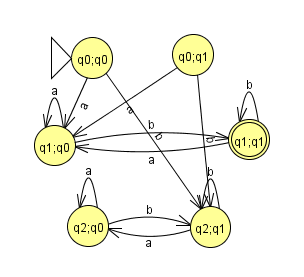
\includegraphics[scale=1]{direkt_a-val_kezdodik_es_b_re_vegzodik.png}
\caption{\label{direkt4} Automata, mely felismeri, ha a szó $a$-val kezdődik és $b$-re végződik}
\end{figure}

Az algoritmus implementációja a forráskódban a \textbf{DFA::and(DFA m1, DFA m2)} metódus.

\subsection{Minimalizálás}
Ha két automata ugyanazt a nyelvet ismeri fel, akkor azt mondjuk, hogy ekvivalensek. Mint ahogy azt látni fogjuk, egy adott nyelvhez több olyan automatát is fel tudunk írni, amely felismeri azt.

Ahogyan fentebb leírtam, képesek vagyunk ilyenkor felismerni két különböző automatáról, hogy ekvivalensek és ez nagyon fontos a feladatkiértékelésnél, de ennél még többet is tudunk. Méghozzá azt, hogy ezen ekvivalens automaták között van egy legkevesebb állapotból álló, úgynevezett minimális automata, és az ekvivalens, de különböző állapotszámú automatákat mind le tudjuk redukálni erre az egyedi, minimális automatára.

Ez azért hasznos, mert így nem kell feleslegesen nagy és bonyolult automatákkal dolgoznunk. Ez egyrészt akkor jó, amikor szemrevételezéssel szeretnénk valamit belátni egy automatáról, másrészt akkor, amikor számítógéppel dolgozunk vele, mert kevesebb állapottal a gép is gyorsabban dolgozik.

\textbf{Definíció.} Egy $M = (Q, \Sigma, \delta, q0, F)$ automata minimális, ha bármely, vele ekvivalens $M' = (Q', \Sigma, \delta', q'0, F')$ automatára $||Q|| \leq ||Q'||$ teljesül.

A minimalizálást két lépésben végezzük:
\begin{enumerate}
\item Eltávolítjuk az elérhetetlen állapotokat, melyekbe az automata sosem juthat el. Ezek nyilvánvalóan feleslegesen vannak benne.
\item A megmaradt automatában megvizsgáljuk melyek azok az állapotok, amelyek összevonásával a felismert nyelv nem változik, majd összevonjuk ezeket.
\end{enumerate}

Az algoritmust egy példán keresztül szemléltetem.

\begin{figure}[H]
\centering
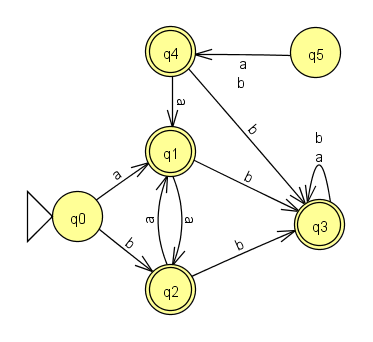
\includegraphics[scale=0.8]{min_kezdo.png}
\caption{\label{mini1} Az automatánk, amelyet minimalizálni szeretnénk}
\end{figure}

Először tehát eltávolítjuk az elérhetetlen állapotokat. A \ref{mini1} ábrán a $q4$ és $q5$ állapotok ilyenek, hiszen a $q0$ kezdőállapotból sehogy nem lehet hozzájuk eljutni.

Ennek a módszere a következő:
\begin{enumerate}
\item Gráfbejáráshoz teljesen hasonló módon a kezdőállapotból kiindulva bejárjuk az 
automatát: Minden állapotnál minden betű állapotátmenetének irányába el kell mennünk. Ezeket a még hátralevő feladatokat egy veremben tároljuk.
\item Eközben listát készítünk arról, mely állapotokban jártunk már. Ezzel azt is elkerüljük, hogy ugyanazt az állapotot kétszer ellenőrizzük, hiszen ahol jártunk már, azt nem kell.
\item Ha a verem kiürült, akkor már minden elérhető állapotban jártunk. Azok az állapotok, amelyeket nem érintettünk, elérhetetlenek.
\item Az elérhetetlen állapotokat töröljük az automatából.
\end{enumerate}

\begin{figure}[H]
\centering
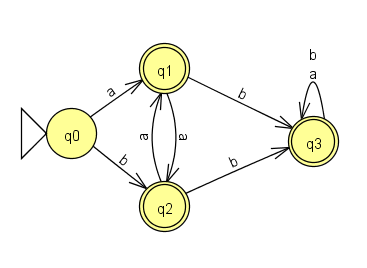
\includegraphics[scale=0.8]{min_feleselhagyott.png}
\caption{\label{mini2} Az elérhetetlen állapotok elhagyása után előálló automata}
\end{figure}

Ezután meg kell állapítanunk, hogy melyek azok az állapotok, amelyek összevonhatóak. Ehhez a következő rekurzív összefüggést kell használnunk:
\begin{enumerate}
\item Először csak annyit tudunk, hogy ha egy $q$ állapot végállapot, és egy $p$ állapot nem végállapot, akkor ők biztosan különböznek és nem vonhatóak össze, ezzel eredendően két halmazra bontjuk az állapotainkat.
\item Ha egy $k$ állapot és egy $t$ állapot valamely betűre nem ugyanabba az állapothalmazba megy át, akkor $k$ és $t$ biztosan különböznek (hiszen biztosan különböző helyre mennek), ezért $k$ és $t$ nem maradhatnak egy halmazban.
\end{enumerate}

Ezen összefüggések alapján az algoritmus a következő:
\begin{enumerate}
\item Az algoritmus során az állapotainkat halmazokra szeretnénk bontani, amelyben nyilvántartjuk, melyek azok az állapothalmazok, amelyek egymástól biztosan különböznek. Ehhez fölveszünk egy táblát, amiben tároljuk melyik állapot éppen melyik halmazban van.
\item Ebbe a táblába először 2 halmazt veszünk fel, azokat az állapotokat amelyek végállapotok, és azokat, amelyek nem.
\item Ezután minden állapoton végigmegyünk és szétválogatjuk őket az alapján, hogy a betűnkénti kimenő állapotaik alapján milyen halmazokba vannak átmeneteik. Ezzel az eddigi halmazaink tovább bomlanak, és ezeket a változásokat fölvesszük a táblánkba is.
\item A 3-as lépést addig ismételjük amíg már nem bomlanak tovább a halmazaink. Ekkor elmondhatjuk azt, hogy azok az állapotok, akik egy halmazban vannak már biztosan összevonhatóak.
\item Fölépítjük a minimalizált automatát. Minden halmaz egy állapot lesz. A közöttük levő átmenetek bármely bennük levő állapotról leolvashatóak. A kezdő állapot az a halmaz lesz, amiben az eredeti kezdőállapotunk volt. A végállapotok azok a halmazok lesznek, amelyekben az eredeti végállapotok vannak.
\end{enumerate}

\begin{figure}[H]
\centering
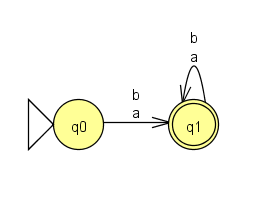
\includegraphics[scale=0.8]{min_minimalizalt.png}
\caption{\label{mini3} Az elkészült minimalizált automata}
\end{figure}

Az algoritmus implementációja a forráskódban a \textbf{DFA::minimize()} metódus.

\subsection{Iteráltat felismerő automata}
Az iterációt $^*$-al jelöljük. Például $ab^*$ azt jelenti, hogy akárhány darab $ab$ egymás után. Akár 0 is. A cél itt az, hogy kapunk egy automatát és állítsuk elő az iteráltját.

Ez a konstrukció nem annyira fontos, de jó példa arra, hogy egy algoritmus sokszor leírható más problémákra, algoritmusokra való visszavezetéssel. Ilyen az is amikor már csak annyit írok, hogy bejárjuk az automatát, mint egy gráfot és közben csinálunk valamit és ilyen lesz ez is. Itt az iterált automatát, mint $\epsilon$(epszilon)-átmenetes automatát fogom felírni.

\begin{figure}[H]
\centering
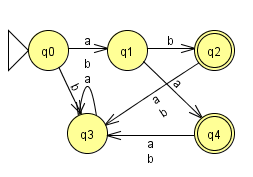
\includegraphics[scale=1]{iter_ab_vagy_aa.png}
\caption{\label{it1} Automata, amely felismeri, ha a szó $aa$ vagy $ab$}
\end{figure}

A \ref{it1} ábrán látható automatára szeretnénk tehát felírni egy olyan automatát, amely felismeri az iteráltját, vagyis az $[aa+ab]^*$ -ot (élőszóban: \textit{aa vagy ab, akárhányszor egymás után}).

Ezt egyszerűen megtehetjük $\epsilon$ átmenettel. Egy $\epsilon$ átmenet annyit jelent, hogy egy állapotból a másikba az automata betű beolvasás nélkül is tud lépni. Az $\epsilon$ átmenetet a JFLAP-ben $\lambda$ jelöli. Minden $\epsilon$ átmenetes automata visszaalakítható rendes véges automatára, de azt az algoritmust már nem tárgyalom itt.

A konstrukció a következő:
\begin{enumerate}
\item A kezdőállapotot célállapottá tesszük (ha még nem volt az). Ezzel garantáljuk azt, hogy 0-szor is szerepelhessen a felismert szó (hiszen az akárhány az lehet 0 is).
\item Minden végállapotból húzunk egy $\epsilon$-átmenetet a kezdő állapotba. Ezzel megengedjük, hogy "visszatekerje" magát az automata az elejére, akárhányszor végzett.
\end{enumerate}

\begin{figure}[H]
\centering
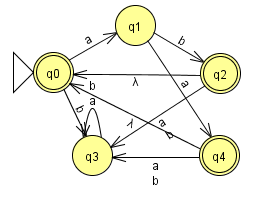
\includegraphics[scale=1]{iter_ab_vagy_aa_eps.png}
\caption{\label{it2} $\epsilon$-átmenetes automata, amely felismeri ha a szó $[aa+ab]^*$}
\end{figure}

A következőkben már csak annyi a teendőnk, hogy az \ref{it2} ábrán látható automatát $\epsilon$ mentesítjük. Ez egy standard eljárás, de nem annyira egyszerű. Itt nem tárgyalom.

\begin{figure}[H]
\centering
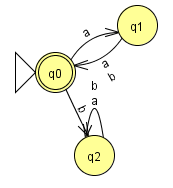
\includegraphics[scale=1]{iter_ab_vagy_aa_kesz.png}
\caption{\label{it3} Az $\epsilon$-mentesített elkészült automata}
\end{figure}

Az algoritmus implementációja a forráskódban a \textbf{dfabuilder::star(DFA dfa)} függvény.

\chapter{Véletlen-generálás}
\section{Bevezetés, procedurális generálás}
A procedurális generálás egy lazán definiált fogalom, általában olyasmit takar, hogy egy függvénynek a kimenetét számítógéppel számoljuk, mert kézzel az idő és pénzigényes lenne, az általános programozástól azonban az különbözteti meg, hogy itt nem az inputot nehéz outputtá alakítani(mint egy utazóügynök problémánál), hanem az output nagyon nagy vagy sokféle lehet és ezt nehéz kézzel előállítani.

2 fő fajtáját ismerjük gyakorlatban:
\begin{enumerate}
\item Az output csak 1 féle lehet, de az az általunk kivánt reprezentációval nagyon nagy:
Ilyenek például a fraktálok, melyeket kézzel kirajzolni nagyon időigényes (főleg a megfelelő matematikai precizitással) , ám géppel könnyű. De például ide sorolhatunk akár egy összetett 3D nyomtatást is.
\item Az output egy nagy halmaz, vagy annak egy véletlen eleme:
Ilyen a játékokban egy véletlen pálya,vagy textúra generálása. De például egy gráf feszítőfái közül egy tetszőleges előállítása is. Ezt a fajtát véletlen-generálásnak hívom.
\end{enumerate}
A továbbiakban kizárólag a véletlen-generálással és annak társproblémáival fogok foglalkozni.

\section{Alapfeladat}
\textbf{Definíció.} $G = (A,K,E)\rightarrow H$, ahol
\begin{itemize}
\item $A$ egy jól definiált alaphalmaz pl: gráfok,automaták,textúrák.

\item $K$ korlátozások halmaza $A$ alaphalmazon, pl. ha $A$ a gráfok halmaza:
\begin{itemize}
\item A gráfban legyen legalább 2 kör, amelyeknek van közös pontja.
\item A csúcsok száma legyen legfeljebb 15 és mindenképp 3-al osztható.
\end{itemize}
Ezen feltételeknek megfelelő elemek az $A$ alaphalmaznak egy szűkebb részhalmazát alkotják.

\item $E$ egy ekvivalencia reláció, pl: 2 gráf akkor egyenlő, ha izomorfak.

Ezen reláció alapján lesznek elemek az $A$ alaphalmazban, melyek a definíció szerint különböznek, de a reláció alapján ekvivalensek.

\item $H$ az $A$ alaphalmazból a korlátozások teljesítésével előálló szűkebb halmaz amelyben minden elem az $E$ ekvivalencia reláció szerint egyedi.
\end{itemize}

A véletlen-generálás eredménye a $H$ halmaz egy véletlenszerűen választott eleme.

Az alapfeladat megoldásának a következő három fontos jellemzője van:\\

\textbf{Helyesség:} Minden $H$-beli elem $A$-beli is, és teljesíti a korlátozásokat.

\textbf{Teljesség:} $H$-ban az összes $A$-beli, a korlátozást teljesítő elem megtalálható.

\textbf{Egyediség:} $H$-ban nincs két elem ami az $E$ reláció alapján ekvivalens. Ez azt is jelenti, hogy a véletlenül választás egyenletes eloszlású.\\

Ez a feladat nagyon nehéz, általában ennek egy könnyített (relaxált) változatát elegendő lesz megoldanunk.

Fontos megjegyezni, hogy ha a halmaz végtelen, nem fogunk tudni belőle egyenletes eloszlással választani. Viszont ha lemondunk az egyenletes eloszlásról, akkor tudunk. Pl.: véletlen egész szám generálás:

$i=1$-ről indul majd 0.5 eséllyel befejezzük és visszatérünk $i$-vel, 0.5 eséllyel viszont $i+=1$ és újra. Ez elméletileg bármely számot kiadhat.

Gyakorlatban általában egy végtelen halmaz végesre korlátozásával fogunk dolgozni. Méghozzá sokszor triviálisan: Tehát például minden legfeljebb 30 elemű gráf.

\section{Ekvivalenciák}
Korábban már említettem, hogy a véletlen generálásnak bemenete lesz egy ekvivalencia reláció is. Ez azért fontos, mert sokszor egy halmazban rengeteg, akár végtelen sok elem van, melyet generálhatunk, de ezek közül rengeteg lényegében ugyanaz, és szeretnénk a generálás során legalább nagyjából elérni azt, hogy változatos elemek legyenek generálva.

Erre való az ekvivalencia relációnk. Pár példa az automaták ekvivalencia relációira:

\begin{itemize}
\item \textbf{Definíció szerinti ekvivalencia.} Ez a legáltalánosabb. Minden definícióhoz tartozni fog valamilyen reprezentáció, ami 1:1 kapcsolatban áll vele. Ezeket a reprezentációkat akár a memóriában binárisan összehasonlítva el tudjuk dönteni, hogy ekvivalensek-e.
\item \textbf{Izomorfizmus.} Ha azt szeretnénk, hogy azok az automaták, amelyek pontosan ugyanúgy néznek ki, csak a címkéik vannak felcserélve ne szerepeljenek többször a generált halmazban akkor ezt használjuk.
\item \textbf{Felismert nyelv szerinti ekvivalencia.} Ilyenkor azok az automaták, amelyek pontosan ugyanazt a nyelvet ismerik fel, ekvivalensek lesznek. Itt voltaképp nem akarunk olyan automatákat generálni, amelyeknek a minimalizáltja izomorf.
\item \textbf{Egyéb logikai tulajdonság szerint.} Megadhatunk bármilyen tulajdonságot, például azt, hogy az ugyanannyi állapottal rendelkező automaták ekvivalensek legyenek. Nyilván ilyenkor nagyon különbözőek lehetnek, de ha számunkra ez a lényeg, akkor lényegében ugyanazok.
\end{itemize}

Az ekvivalenciák kérdéséhez tartoznak a nyelvtani szinonimák is, melyek kezelése nagyon nehéz, nem is sikerült a típusos generálásban jól kezelnem ezt a kérdést.

\section{Elhelyezkedés a számítástudományban}
A véletlen-generálás közel áll számítástudományi alapproblémákhoz:
\begin{enumerate}
\item Eleme-e probléma(=kiértékelés): Kapunk egy $B$ halmazt és egy $b$ elemet, döntsük el, hogy $b\in B$! (nekünk most ez azt jelenti, hogy döntsük el egy kapott gráfra, például, hogy kielégíti-e a felsorolt feltételeket, tehát eleme-e a szűkített halmaznak)
\item Van-e eleme(=kielégíthetőség): Kapunk egy $C$ halmazt, kérdés hogy $C$-nek van-e egyáltalán egyetlen eleme. Itt az a kérdés, hogy a feltételek együttesen kielégíthetőek-e valahogy, tehát üres-e a szűkített halmaz, vagy sem.
\item Generálj egy tetszőleges elemet(=modellkeresés): Ez ugyanaz, mint a 2, csak itt arra is kíváncsiak vagyunk, hogy melyik az az elem, ami kielégíti a feltételeket.
\item Adj meg egy optimális elemet(=optimalizálás): Ez hasonló, mint 3, csak itt a szűkített halmaz elemei nem csupán kielégítik a feltételeket, de van köztük egy olyan reláció is, amely alapján van köztük jobb és rosszabb, és mi a legjobbat/legrosszabbat keressük.
\item Hány elemű a halmaz(=számosság): Adjuk meg hány olyan elem van ami kielégíti a feltételeket.
\item Enumeráció: Soroljuk fel a halmaz összes elemét (ha minden elemet csak egyszer akarunk, akkor az Egyedi Enumeráció). Itt mi minden olyan elemet listázunk, akik megfelelnek a feltételeknek.
\end{enumerate}
Ezek közül az enumerálás áll a legközelebb hozzánk. Hiszen, egy véges halmaz elemeit fel tudjuk sorolni, és mindhez tudunk társítani egy számot, így ebből a listából egy véletlen egész számot generálva indexeléssel meg tudjuk oldani a véletlen-generálási problémát. Ez működni fog akkor is, ha a halmaz végtelen, de sorba rendezhetőek az elemei (persze, mint előbb írtam ez már nem lesz egyenletes).

Tehát mondhatjuk azt, hogy minden véletlen-generálás előáll valamilyen enumerációs algoritmusból, ahol a döntések során véletlenszerűen választunk, így ha van egyedi enumeráló algoritmusunk, akkor azzal egyszerű véletlen-generálni. Viszont anélkül is lehet, de ott az általános probléma nehezebb lehet (ha egyáltalán megoldható).

\section{Véletlen-generálás a gyakorlatban}
A gyakorlatban ma már sok helyen használják, például a SpeedTree nevű cég realisztikus fákat, növényzetet generál hollywoodi filmekhez.

Általában az a cél, hogy részletes tájat, pályát, világot hozzunk létre anélkül, hogy minden apró részletet egy embernek kéne létrehoznia. Lehet fel sem tűnik, de a fű brush, amivel pályaszerkesztőkben a füvet tudjuk \textit{"felszórni"} a földre, az is egy véletlen-generálás. De persze azt, hogy hol legyen a fű, a pálya készítő dönti el, és ez így egy félautomata módszer, ami időt és pénzt takarít meg.

Vannak viszont olyan játékok is, amelyek alapjaiban épülnek a véletlen-generálás sokszínűségére. Ilyen pl. a Minecraft, vagy a No Mans Sky, ahol egész pályák teljes elrendezését generálják véletlenszerűen. Ezekből viszont még sokszor érezni, hogy hiányzik az emberi kéz.

\section{Módszerek véletlen-generáláshoz}
A következőkben pár módszert sorakoztatok fel, amelyeket interneten talált anyagokból\cite{Mary} és eddigi ismereteimből raktam össze.

\pagebreak
\subsection{Backtrack és teljes rendezés}
A generálás során az egyediség garantálásának legjobb módja a backtrack módszer.
\begin{figure}[H]
\centering
\begin{forest}
[$Gen$
	[$H$
		[$A$]
		[$\overline{A}$]	
	]
	[$\overline{H}$
		[$B$]
		[$\overline{B}$]
	]
]
\end{forest}
\caption{\label{backtrack} Generált halmazok üres metszetének szemléltetése az ágakon}
\end{figure}
Itt a generálást, mint független döntések sorát tekintjük, ahol az egyediséget az ábrán látható módon úgy tudjuk garantálni, hogy ha például a $H$ irányban generált elemek biztosan nem találhatóak meg a $\overline{H}$ irányban levőek között és fordítva. Ekkor a fa levelei biztosan egyediek lesznek. Természetesen ez nem csak két irányra működni, hanem többre is, ilyenkor az irányokban legenerálható halmazok metszete üres kell, hogy legyen. Ez a többes elágazás általában for ciklusként jelenik meg a kódban.

Felmerül azonban a kérdés, hogy egy adott esetben, hogyan írjuk fel a generálást, mint független döntések sorozatát (már ha lehet). Erre fogjuk használni a teljes rendezés nevű módszert, ahol a lehetséges sokféle döntésünket valamilyen mérce alapján rendezett sorba állítjuk. Ezt egy példán keresztül jobb látni, ezért itt adok egy algoritmust véges automaták enumerálására. A lépései a következők:

\begin{enumerate}
\item Először az 1 elemű automatákat generáljuk, majd a 2, majd a 3. Így mindet le fogjuk tudni és egyszerre elég egy méretet kezelni. Ez már itt egy teljes rendezés.
\item Az adott $n$ elemű automata generálásánál láthatóan véges sok opció van. Letesszük először mind az $n$ állapotot.
\item Sorba vesszük az összes lehetséges átmenetet aszerint, hogy állapotonként abból az állatból melyik betűre melyik állapotba megy.
\item Ezen rendezések alapján már rekurzívan egybeágyazott for ciklusokkal végigmehetünk a lehetséges döntéseken.
\item Végezetül a célállapotok halmaza az állapotoknak egy részhalmaza, a kezdő állapot pedig az egyik megválasztott állapot lesz.
\end{enumerate}

Az egyediség ennél a módszernél garantált, a teljesség és a helyesség viszont nehezebb.

\subsection{Más ekvivalenciákra történő kiterjesztés}
Az előző módszer hátránya, hogy olyan automatákat is gyárt, amelyek különböznek de izomorfak.

\begin{figure}[H]
\centering
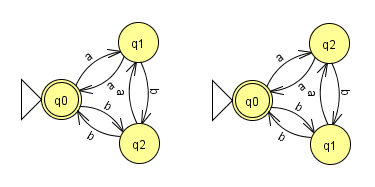
\includegraphics[scale=1]{equiv.png}
\caption{\label{izomorf} Két véges automata, melyek különböznek, de izomorfak}
\end{figure}

Mint ahogyan az ábrán is látható, a $q1$ és $q2$ címkék cseréjével megkapjuk az egyik automatából a másikat. Az előző algoritmus mind a kettőt enumerálja. Azonban ha a generáló algoritmusunk más ekvivalenciát kap, például azt, hogy izomorfságra egyediek legyenek az automaták, akkor már csak az egyiket szeretnénk megtartani. Ezt valahogy úgy tudnánk elérni, hogy ha a generálás során a $q0$-ból $q1$-be behúztunk egy $a$ betűs átmenetet, akkor később már a $q0$-ből $q2$-be ne húzhassunk ilyet (hiszen pont így keletkezik a duplikátum).

Az általános trükk itt az, hogy a generálás minden pillanatában azokat a lehetőségeket, amelyek nem egyediek, egy halmazként tekintjük, amelynek tetszőleges elemét választjuk ki. Például:

Amikor a fenti ábrán látható automata generálása során még csak a 3 állapot van lerakva, akkor az első dolgunk a $q0$ megjelölése után, hogy eldöntsük, a $q0$ állapotból $a$ betű hatására hova szeretnénk átmenetet. Definíció szerinti esetben itt 3 lehetőségünk lenne a 3 állapottal. Azonban mivel itt izomorfizmus a relációnk, itt a $q1$ és $q2$ jelen pillanatban pontosan ugyanúgy néz ki, hiszen egyiküknek sincs semmilyen éle, ezért őket $\{q1,q2\}$ halmazként kezeljük, így a választásunk a $q0$ és a $\{q1,q2\}$ között dől el. A következő lépésben pedig már egyedi lesz mind a 3 állapot.

\pagebreak
\subsection{Szupergráf}
A szupergráf módszernél egy, a generálandó halmaz tetszőleges eleméből indulunk ki, melyből aztán ekvivalens átalakításokkal más elembe jutunk.

Ez a módszer garantálja a helyességet, viszont az egyediséget, teljességet nehéz garantálnia.

Az egyediséget ennél a módszernél az algoritmus tárhelyének korlátozásával próbálhatjuk meg elérni.

\subsection{Nemdeterminisztikus}
Ha nincs egy bonyolult és helyes algoritmusunk a generáláshoz, akkor még mindig folyamodhatunk a következő módszerhez:
\begin{enumerate}
\item Legenerálunk egy elemet valamilyen buta módszerrel.
\item Ellenőrizzük, hogy az elem helyes-e (benne van-e a generálandó halmazban) és ha nem az, akkor eldobjuk.
\end{enumerate}

Ez a módszer sok esetben teljesen jól működik, tipikusan akkor hasznos, ha van egy tulajdonság, amit könnyű ellenőrizni, ritkán fordul elő és nehéz lenne garantálni. Ilyen például a feladatgenerálásnál az üres automata. Ritkán fordul elő, ezért ha észre vesszük a generálás végén, hogy üres automata, akkor eldobjuk és újat generálunk.

Amikor viszont a sok helytelen megoldás között alig van helyes, a nemdeterminisztikus módszer túl lassú lesz.

Fontos azonban tudni, hogy a SAT problémánál a lehetséges kielégítő értékadások enumerációját csak nemdeterminisztikus módszerrel tudjuk generálni (ha P$\neq$NP) .

\chapter{Típusos generálás}
\section{Bevezetés és definíció}
A fentebb vázolt módszerekkel szemben, vagy inkább azokat kiegészítően a típusos generálás egy másik megközelítése a problémának. Ehhez azt kell észrevenni, hogy a legtöbb végtelen halmaz leírható véges sok atom végtelen kompozíciójával.

Ilyen például az, hogy minden ítéletlogikai függvény felírható NAND kapuk kompozíciójával, tehát ez a halmaz egyetlen elemből típusosan generálható.

De ilyenek például a reguláris nyelvek is, amelyeket a véges input abc-ből az unió , konkatenáció és iteráció műveletekkel végtelenül komponálva megkapjuk az egész halmazt. Tehát egy 3 elemű abc-jű nyelvet 6 atom kompozíciójával típusosan le tudjuk generálni.

Előfordulhat azonban az, hogy egy halmazt nem tudunk véges sok atom kompozícióval generálni. Ilyenek például a természetes számokra teljesülő elsőrendű állítások halmaza és más egyéb nem kompakt halmazok. Ugyanakkor ezen esetekben is hasznos lesz a típusos generálás, mert ugyan az algoritmus nem lesz teljes, megfelelő számú atommal kellően változatos és hasznos eredményt kapunk. A Peano axiómák is pontosan ezt teszik.

Felmerülhet később a kérdés, hogy ha a reguláris nyelveket, és így a véges automatákat három művelettel és az abc-vel le tudjuk generálni, akkor mi értelme van húszféle atomot használni. A válasz pedig az, hogy az automatás feladatok nehézsége pont az, hogy valamilyen logikai összefüggést a hallgató az automaták "nyelvére" tudjon fordítani, és ehhez nem elég automatát generálni, de azt is látnunk kell, hogy milyen nyelvi, matematikai tulajdonságokat teljesít az automata. Így a típusos generálás képes hidat alkotni a generált halmaz, és a halmaz elemeiről megfogalmazható tulajdonságok között.\\

\textbf{Definíció:} $T = (A,R)\rightarrow G$, ahol
\begin{itemize}
\item $A$ az atomok halmaza
\item $R$ szabályok halmaza, amelyek megadják, mely atomok kombinálhatóak egymással (ez a típusrendszer)
\item $G$ a generált halmaz, amely az $A$ atomok $R$ szabályok mentén történő minden lehetséges kompozícióját tartalmazza.
\end{itemize}	

A véletlen-generálás eredménye $G$ egy véletlen eleme.

\section{Véges automatás feladatok típusos generálásának folyamata} 
A cél az, hogy a feladatszövegeket, és azok megoldását egyszerre generáljuk le, ehhez egy többlépcsős generáló folyamatot használunk:
\begin{enumerate}
\item Véletlen generálunk egy fát, amely teljes egészében leírja a feladatot.
Ezt a lentebb felírt szabályokkal, mint generatív nyelvtannal megadott CF nyelv véletlenszerű kifejtésével tesszük.
\item A generált fát lefordítjuk véges automatára, tehát csúcspontonként bejárva a fát, alulról felfelé fölépítjük azt a véges automatát, amely a feladat megoldása. Ezzel tudjuk majd ellenőrizni, hogy a feladatra beérkezett megoldás jó-e.
\item A generált fát lefordítjuk magyar nyelvű feladatszövegre. Ezt a szöveget adjuk a diákoknak.
\end{enumerate}
Ez a többlépcsős folyamat megbonyolítja a generálást azonban igen nagy előnyökkel is jár, mert ha kifejtés közben generálnánk a szövegeket és az automatákat, akkor ők nem látnák a (még meg nem épült) fát maguk körül.

Olyan ez, mint amikor mielőtt megszólalunk, átgondoljuk, hogy miről is szeretnénk beszélni, és csak akkor kezdünk el beszélni, amikor ez már megvan. Tehát fölépítjük a szemantikát teljesen mielőtt a mondatot elkezdenénk fölépíteni, így nem akadunk meg.

Ennek nagy előnye például a magyar mondat generálásánál, hogy a második lépcsőfokon hozzá tudunk adni környezetfüggő viselkedést az eredetileg környezetfüggetlen nyelvtannal generált szerkezethez. Így a toldalékokat is sokkal könnyebb kezelni. Továbbá az is lényeges előny, hogy a generált fának semmivel nem kell bonyolultabbnak lennie, mint ami már egyértelműen definiálja az etalonnak szánt véges automatát és a magyar nyelvű feladatleírást. Ennek következtén a véletlen generálás tulajdonságai is a fa generálásánál dőlnek el.

Az algoritmus implementációja a forráskódban a \textbf{CFGenerator()} függvény.

\pagebreak
\section{A típusos generálás főbb tulajdonságai}
A típusos generálás a tökéletes generálás feltételeit nem teljesíti, azonban számunkra még így is hasznos.\\

\textbf{Helyesség:} A típusos generálás mindig helyes, mert a faszerkezet feldolgozása során garantálni tudjuk ezt.

Jelen esetben is az, mert a konstrukciók folyamán rekurzívan garantáljuk, hogy minden amit generálunk, véges automata. Továbbá a magyar nyelvű feladatleírásnál is garantáljuk a mondatok nyelvtani helyességét a szabályokkal.\\

\textbf{Teljesség:} A típusos generálás általában nem teljes, ennek oka, hogy csak azokat a véges kombinációkat tudja, amiket megadtunk neki a fát felépítő szabályoknál. Ez azért nem baj, mert mint ahogy fentebb említettem nem szokott probléma lenni, hogy a véges generálás nem tud mindent generálni, ha tud elegendően sok variációt generálni.

Jelen esetben azonban lehet teljes is a véges automatákat tekintve, hiszen tudjuk, hogy a véges automaták osztálya megegyezik a reguláris nyelvekével, márpedig bármely reguláris nyelvet felírhatunk az abc-beli betűkből, az üres nyelvből, és az üres string alkotta nyelvből kiindulva konkatenációval, unióval és Kleene star-al. Az általam felírt generálási szabályok nem teljesek, mert korlátozva van a generálás szélessége és mélysége a feladatok érthetősége miatt, de ennek a föntebb leírt okokból nincs igazán jelentősége.\\

\textbf{Egyediség:} A típusos generálás általában nem egyedi és nehéz azzá tenni, viszont lényeges előnyökkel jár ha legalább nagyjából sikerül egyedivé tenni. Hiszen ekkor kevesebb valószínűséggel generál például feladatokat amik ugyanazok csak máshogy vannak megfogalmazva (szinonimák) .

Jelen esetben sem egyedi a generálás, de ezzel nincs különösebb probléma.

\section{Implementált típusok felsorolása}
\begin{forest}
for tree={%
    folder,
    grow'=0,
    fit=band,
  }
[Szimbólumok
[W: Szóra vonatkozó állítás
    [C: Tartalmaz <S>-t mint részszó]
    [D: Bármely <N> egymás utáni betűje tartalmaz <Y> darab egymás utáni <B>]
    [E: <W> és <W>]
    [F: <Y> darab egymás utáni <S>]
    [K: Tartalmaz <Y> darab <S>-t]
    [L: \textit{n = <P> | n <J>}]
    [O: <W> vagy <W>]
    [S: Fix szó (pl. aba)]
    [T: Nem <W>]
    [U: Minden <B> után áll egy <B>]
    [V: <S>-re végződik]
    [Z: <S>-el kezdődik]    
  ]
  [B: Abc-beli betű]
  [P: Szóval kapcsolatos számlálós kifejezés (pl. Wa - Wb)]
  [Y: Számra vonatkozó állítás
    [Q: Pontosan <N> darab]
    [R: Legfeljebb <N> darab]
    [\$: Legalább <N> darab]       
    [J: Véges tulajdonságra vonatkozó állítás
      [X: Páros]
	  [$|$: Páratlan)]
	  [H: Osztható <N>-el]
	]    
  ]
  [N: Fix szám (pl. 3)]  
]
\end{forest}

\begin{forest}
for tree={%
    folder,
    grow'=0,
    fit=band,
  }
[Segédjelek:
	[A : Fix szó generáló segéd]
	[M : Fix szám generáló segéd]
	[I : Fix szám generáló segéd]	
	[\& : P-hez segéd]
	[e : Előre]
	[h : Hátra]
	[z : Egyhelyben]	
  ]
\end{forest}

\section{Szimbolikus entitások}
Köznyelvben és matematikában is gyakran előfordul, hogy az entitás, amiről valamit állítunk nem közvetlenül és azonnal meghatározott. Például \textit{"Ott állt előttem valaki, aki kabátban volt és angolul beszélt."}, vagy \textit{"x = 5*c , ahol c a legkisebb eleme a tömbnek."}, ezt nevezem itt szimbolikus entitásnak. Ezekkel kapcsolatosan sokféle nyelvi elem van, amire szükség van egy típusos generálásnál, a következőkben a legfontosabbakról írok.

\subsection{Általánosítás}
Amikor hétköznapi értelemben számokról beszélünk, akkor olyasmik jutnak eszünkbe, hogy 5, vagy 0.34, esetleg $\pi$. Ha viszont például van egy olyan mondatunk, hogy\\
1: \textit{„Gondoltam egy szóra, melyben az ’a’ betűk száma 3.”}\\
, akkor  érezhető, hogy a következő mondat:\\
2: \textit{„Gondoltam egy szóra, melyben az ’a’ betűk száma 5.”}\\
nagyon hasonló hozzá. Hasonló a mondat alakja, és a jelentése is (szemantika).

De nézzük a következő két szót:\\
\textit{„mivel”} és  \textit{„mível”}, ezen szavaknak az alakjuk hasonló, ám teljesen mást jelentenek.

Persze mondhatjuk, hogy a világon lehet egy olyan nyelv, amelyben ez a két szó jelentése is hasonló és ez a téma nagyon összetett, mivel az élő nyelv folyamatosan változik, a szavak jelentése, azok szemantikája, vagy akár alakja változhat egy adott nyelven belül is.

Ezért fontos bevezetni a szemantikai leíró fogalmát:

A \textbf{szemantikai leíró} egy algoritmust ír le, amely felismeri, hogy az inputja eleme-e egy meghatározott halmaznak. Ezt a leírót a megfelelő gépbe beadva a gép eldönti, hogy eleme-e az input a halmaznak.

Továbbá bevezetjük az értelmezés fogalmát:

Az \textbf{értelmezés} egy algoritmus ami egy mondatról egy szemantikai leíróra fordít.
Tehát egy adott értelmezésben az 1-es mondatot lefordítva kaphatjuk a következő szemantikai leírót:
\begin{verbatim}
INPUT: word
int count = 0;
for(char c: word){
	if(c == ’a’) count++;
}
if(count == 3) ACCEPT;
else REJECT;
\end{verbatim}

A 2-es mondathoz tartozó leíró pedig:
\begin{verbatim}
INPUT: word
int count = 0;
for(char c: word){
	if(c == ’a’) count++;
}
if(count == 5) ACCEPT;
else REJECT;
\end{verbatim}

Pongyolán azt mondhatjuk, hogy két mondat jelentése hasonló, ha az adott értelmezés mellett a szemantikai leíróik részben hasonlítanak.

Ennél pontosabban megfogalmazva, ha két mondat jelentése hasonló, akkor létezik olyan leíró, amely megfelelően paraméterezve ekvivalens mindkét -az adott értelmezésben lefordított- leíróval. 

Vagy talán még szebben úgy is mondhatjuk, hogy a paraméternek, mint szabad változónak létezik olyan megkötése, amely az 1-es leíróval megegyező működést okoz, és létezik olyan megkötése is, amely a 2-es leíróval megegyező működést okoz.

Itt például:

\begin{verbatim}
INPUT: word, N
int count = 0;
for(char c: word){
	if(c == ’a’) count++;
}
if(count == N) ACCEPT;
else REJECT;
\end{verbatim}

Ilyenkor ezt a leírót a két mondat \textbf{általánosított szemantikai leíró}jának nevezzük.
 
\subsection{Indirekció}
A következő mondat:\\
3: \textit{„Gondoltam egy szóra, melyben az ’a’ betűk száma kisebb, mint 3.”}

szintén nagyon hasonlít az utóbbi 1-es mondatra:\\
1: \textit{„Gondoltam egy szóra, melyben az ’a’ betűk száma 3.”}

Ők is azért hasonlítanak, mert van közös általánosított leírójuk:

\begin{verbatim}
INPUT: word, numberPredicate()
int count = 0;
for(char c: word){
	if(c == ’a’) count++;
}
if(numberPredicate(count) == true) ACCEPT;
else REJECT;
\end{verbatim}

Ahol a \textit{numberPredicate(k)} az $k$ számnak egy tulajdonságát ellenőrzi. Az 1-es esetén ez a tulajdonság: $A == 3$, míg a 3-asnál $A < 3$.

Azt, hogy az értelmezés során indirekció történik, a mondatban is meg szokták jelölni, pl. így:\\
3b: \textit{„Gondoltam egy szóra, melyben az ’a’ betűk száma A, ahol A kisebb, mint 3.”}\\

Mivel a fentebbi leírók C nyelven íródtak és az őket futtató gép egy számítógép (C fordító->bináris processzor utasítások), úgy tűnhet, hogy az indirekciókat megvalósító leírók megvalósítása egy triviális dolog. Ez nincs mindig így. Nézzük a következő példát:\\
4: \textit{„Gondoltam egy szóra, melyben az ’a’ betűk száma kisebb, mint A, ahol A kisebb, mint 3.”}

Ez egy valid indirekció, de a mondatot még értelmezni is nehéz.\\

Ha explicitté tesszük az egész kifejezést ez jön ki:\\
4b: \textit{„Gondoltam egy szóra, melyben az ’a’ betűk száma B, ahol B kisebb, mint A és A kisebb, mint 3.”}\\
Tehát $0 \leq B < A$ és $A < 3$, ahol $A$ és $B$ szabad változók, vagyis bármilyen értéket felvehetnek.

A következő kombinációk lehetségesek \textit{(A,B)} párokkal felírva:

\textit{(1,0),(2,0),(2,1)}, tehát a $B$ (vagyis az $a$ betűk száma) a $\{0,1\}$ halmazból kerülhet ki.
Ezt C kódban sem könnyű kezelni. Ugyanis, ha ezt az indirekciót implicitté tesszük a mondatban ezt kapjuk:\\
4c:\textit{”Gondoltam egy szóra, melyre van olyan szám, ami az ’a’ betűk számánál nagyobb, de 3-nál kisebb.”}\\
Ez pedig egy elsőrendű logikai kifejezés.

C kódban az ilyeneket kezelhetjük úgy, hogy kötött B-re és szabad A-ra rezolúcióval megoldjuk a kielégíthetőséget. Vagy akár ezt a folyamatot be is építhetjük magába a kódba. A prolog is hasonlókat csinál, de ebbe most nem megyek bele, mert csupán érinti a témát.

\subsection{Foldok}
Az általánosítások és indirekciók kezelése automatáknál sokkal nehezebb, mert az ilyen paramétereket nem tudjuk csak úgy átadni az automatának, hiszen annak egyetlen paramétere a szó amit felismer vagy nem.

Ezeket a paramétereket bele kell építeni az automatába a konstrukció közben, ezt nevezem itt foldnak.\\

\textbf{Első példa:}

Például ha egy olyan automatát szeretnénk építeni, amely felismeri, hogy szerepel-e a szóban részszóként $aba$, akkor ezt az $aba$-t nem tudjuk csak úgy átadni az automatának. A konstrukció folyamán beépítjük. Ennek legegyszerűbb módja ha egy $\epsilon$ átmenetes automatába  csinálunk 4 állapotot, és 3 átmenetet köztük sorban $a$, $b$, $a$ betűkre. Majd rakunk az elejére és a végére is $\Sigma^*$ csillagot, majd $\epsilon$ mentesítünk és determinizálunk.

Az algoritmus implementációja a forráskódban a \textbf{dfabuilder::contains(DFA\\sym\_word)} függvény.\\

\textbf{Második példa:}

Automata, amely $ab$-t tartalmaz $N$-szer, ahol $N$-re igaz valamiféle predikátum(pl \textit{páros}, $=3$, $>2$, stb). Ezt a predikátumot szintén automatával adjuk meg, ahol a szám növekedésére egy $e$ betűs, nem növekedésére pedig egy $z$ betűs állapotátmenetet teszünk. Ezután kreálunk egy automatát, amely akkor fogad el, ha a szó $ab$-re végződik. Majd a két automatát párhuzamosan futtatva hatványhalmaz konstrukciót csinálunk, ahol az $N$-es automata az $e$-s átmenetén akkor lép, ha az $ab$-re végződős automata végállapotba ér, különben a $z$-s állapotra lép.

Ez logikus is, hiszen ha egy szó $ab$-t $N$-szer tartalmaz, az azt jelenti, hogy a szó beolvasása során az $ab$ $N$-szer lesz az addig beolvasott szó végén.

Az algoritmus implementációja a forráskódban a \textbf{dfabuilder::containsNTimes(DFA nTimes, DFA sym\_word)} függvény.\\

\textbf{Harmadik példa:}

Automata, amelynek minden $N$ egymás utáni betűjére igaz valami predikátum. A predikátumot szintén automatával adjuk meg. Itt először csinálunk minden lehetséges $N$ egymás utáni betűre egy állapotot, majd ezeken az $N$ elemű szavakon futtatjuk a predikátumot, mint automatát. Ha elfogadta, akkor célállapot lesz, ha nem akkor nem. Továbbá minden $N$-nél rövidebb szó automatikusan célállapot, hiszen arra nem vonatkozott a megkötés.

Az algoritmus implementációja a forráskódban a \textbf{dfabuilder::NConsecutive(DFA sym\_word, DFA nmbr)} függvény.\\

A példákból látható, hogy ez egy nagyon fontos része a generálási folyamatnak. Ezért definiálom a fold fogalmát pontosabban is:\\

\textbf{Definíció.} Adott egy probléma, amelyben van legalább egy szabad változó. Adott egy, a szabad változókat megkötő állítás. Foldnak nevezzük azt az algoritmust, ami előállít egy algoritmust, ami megoldja a problémát a változók kötése mellett.\\

Például:

Probléma: $W$ input szó tartalmazza-e $S$ szót.	($S$ itt egy szabad változó, bármi lehet)
Kötő állítás: $S = aba$, vagy $S$ $a$-ra végződik.

Fold: (Probléma, kötő állítás) -> Algoritmus (itt véges automata)

Algoritmus: Eldönti, hogy $W$-nek része-e $aba$, vagy a másik példában, hogy $W$-nek része-e olyan szó ami $a$-ra végződik.\\

Az algoritmusokat a generálás során következetesen véges automatákkal adtam meg, ezzel garantálom, hogy akárhány fold után is olyan nyelv keletkezzen, amely felismerhető véges automatával.

Végezetül egy lista a foldokról (aszerint, hogy mi a kötés) nehézsége szint szerint:
\begin{enumerate}
\item Fix szó
\item Véges szó halmaz
\item Predikátum (=algoritmussal megadott szó, általában végtelen halmazból)
\item Predikátumokból álló logikai kifejezés szabad változó nélkül (=Ítéletlogikai kifejezés)
\item Logikai kifejezés másik kötött változóra történő hivatkozással vagy szabad változókkal (=Első és magasabb rendű kifejezés)
\end{enumerate}

\section{Nyelvi problémák a típusos generálás körül}
A típusos generálás során egy kontextusfüggetlen (cf) nyelv segítségével generálunk szavakat a formális nyelvek órán megismert kifejtő módszerrel. Ez így egyszerű, hiszen egy faszerkezetben kifejthetők a szemantikus elemek, viszont ez korlátokat is jelent.

Ezen korlátok van, hogy \textbf{(1)} elméleti jellegűek, tehát egy bizonyos feladatfajtát nem tudunk megvalósítani. És van, hogy \textbf{(2)} gyakorlati jellegűek, tehát ugyan a feladatot meg tudjuk valósítani, de nehézkes, problémás.

Általánosan a kontextus-független nyelvek korlátja az, hogy nem lehet bennük egy adott elem kifejtésétől függően kifejteni egy másikat.

Mivel a feladatok általánosan a\\
\textit{<valamiről> <állítok valamit>}\\
sémára épülnek ezért egy cf nyelvvel csak úgy tudjuk generálni ha lefixálunk egy típust, például,\\
\textit{<valamilyen mérték, ami egy egész szám és jelöljük n-el>  <n páros>}
\subsection*{Elméletileg sem lehetséges}
A következőt például cf nyelvvel (legalábbis általánosan) nem lehet megcsinálni:\\
$\{ba^ncb^ma | n - m >  5,$ \textit{n páros}$\}$\\
\textit{<miről állítunk> | <mit>} sémában itt a bal oldalon definiáljuk, hogy mi is ez az $n$ és $m$, és ezekre a jobb oldalon szeretnénk valami állítást megfogalmazni, tehát balról jobbra kell, hogy menjen az az információ, hogy van egy $n$ és egy $m$ egész szám. Ez így, ebben a konkrét esetben működhet, hiszen csinálunk egy típust, ahol fixen $n$ és $m$ változókról állítunk dolgokat, de ez általánosan nem megy:\\
$\{ba^ncb^mac^k | n-m > 5,$ \textit{n páros, n + k páratlan}$\}$\\
Ezt már az előző sémával nem tudjuk megcsinálni, mert nem megy át a $k$. Általánosan is az a probléma, hogy a \textit{<miről állítunk>} blokkban keletkeznek a változók amikről állítani szeretnénk valamit és végtelen sok is keletkezhet, erre pedig véges sok típussal nem fogunk tudni felkészülni.
\subsection*{Lehetséges, de a gyakorlatban nehézkes}
Sokat elmond a cf nyelvek korlátozottságáról, hogy ha az abc elemeitől szeretnénk függővé tenni valamilyen kifejtést, azt nagyon nehezen tehetjük meg.

A következő példa ezt jól szemlélteti:\\
$|W|_a - |W|_b + |W|_c$ \textit{páros}

Itt arról van szó, hogy van egy aritmetikai kifejezésünk, amely bizonyos abc-beli betűkből alkotott aritmetikai kifejezés eredményéről állít valamit (itt például azt, hogy páros). Cf nyelvben ezt meg lehet csinálni, de minden alkalommal, amikor az abc-nk változik, az összes segéd-terminálisunkat újra kell írni.

Ezen úgy tudtam segíteni, hogy egy for ciklussal az abc specifikus szabályokat dinamikusan betöltöm a generatív nyelvtanba generálás előtt.

\chapter{A magyar nyelvű feladatszöveg generálása}
Amikor a generált fából a mondatokat összerakjuk, az a legnagyobb nehézség, hogy a mondatok értelmesek legyenek, és ne úgy nézzen ki, mint amit Google fordítóból szedtek ki.

Itt sok apró probléma van, amelyeket egyesével felsorolok.

\section{Toldalékok}
Ahhoz, hogy értelmes mondatok keletkezzenek, fontos, hogy használjunk toldalékokat, és a megfelelő alakban használjuk azokat.

\textit{„A kutya ül a fű.”}, vagy \textit{„4-al osztható”} jellegű kifejezések erősen kétségbe vonnák a feladatok komolyságát.

A megfelelő toldalék választásával nem szokott sok gond lenni. A hangalak egy kicsit problémásabb. Általában a szavak, szótagok magas, mély és vegyes hangrendűségétől függ a toldalékok hasonulása.

Magas hangrendű magánhangzók: e,é,i,í,ö,ő,ü,ű

Mély hangrendű magánhangzók:  a,á,o,ó,u,ú

Egy szó magas hangrendű, ha benne csak magas hangrendű magánhangzók vannak, például:\\ \textit{„kilenc”}, ilyenkor a toldaléka is magas: \textit{„kilenccel”}

Egy szó mély hangrendű, ha benne csak mély hangrendű magánhangzók vannak, például:\\ \textit{„kalóz”}, ilyenkor a toldaléka is mély: \textit{„kalózzal”}

Egy szó vegyes hangrendű, ha benne magas és mély hangrendű magánhangzók is vannak, például:\\
\textit{„Gina”}, ilyenkor a toldaléka mély: \textit{„Ginával”}

Ennél bonyolultabb esetek is vannak a toldalékok hangalakjára, de egyszerűbb esetekben ez működik.

Nekünk viszont nincs szükségünk ilyen bonyolult logikai összefüggések kódolására, hiszen amikre toldalékok kerülnek azok vagy számok (amelyeknek utolsó tizedesjegye 0-9 lehet, tehát véges sok), illetve szavak, melyeknek az utolsó betűjéhez hasonul a toldalék, és ezekből is véges sok van, ezért elegendő egy switch case-el minden lehetőségre kézzel beégetni a toldalékokat.

\section{Negálás}
Magyar nyelvben a negálás nem egyszerűen az, hogy elé rakunk egy \textit{„nem”}-et az állításnak, hiszen akkor olyan kifejezések keletkeznének, hogy \textit{„nem büszke vagyok”}.

Például:\\
\textit{„W ab-vel kezdődik”} $\rightarrow$ \textit{„W nem kezdődik ab-vel”} (tehát a szórend itt változik)\\
\textit{„W-ben az a-k száma osztható 5-el”} $\rightarrow$ \textit{„W-ben az a-k száma nem osztható 5-el”} (a szórend itt nem változik, elég kirakni a \textit{nem}-et)\\
\textit{„Bármely a betű után áll egy b betű”} $\rightarrow$ \textit{„Van olyan a betű, amely után nem áll b betű”} (ez egy elsőrendű kifejezés, ezt még nehezebb értelmesen negálni)

Ezeket az eseteket CF nyelvvel kezelni elég nehéz, de nem lehetetlen, hiszen minden mondatnak kétféle alakja van, a negált és a negálatlan, tehát véges sok variáció van, ezért generálható cf nyelvvel, csak nem célszerű. Erre a célra a kódban az értelmezés során egy \textit{ál}-kontextusfüggő működést raktam be, amely minden negálásnál lefele tol egy jelzést, hogy minden állítás maga tudja eldönteni, hogyan viselkedjen negálás esetén.

\section{Logikai kifejezések}
Amíg egy elsőrendű logikai kifejezésnél természetes a rengeteg egybeágyazott \textit{és}, \textit{nem}, \textit{vagy}, \textit{kvantor} stb. , addig magyar nyelvben ezeket nem lehet csak úgy zárójelezéssel végtelenül halmozni.

Ha pl. azt akarjuk negálni, hogy \textit{„fehér a hó és kék az ég”}, akkor azt úgy szokás, hogy \textit{„nem igaz az állítás, hogy fehér a hó, és kék az ég”}, tehát itt egy indirekciót kell explicit jelölnünk az állításra. Ezt a technikát tetszőleges logikai kapcsolatokra használhatjuk:\\
\textit{„Van egy állításom, hogy piros a hó és zöld az ég, és van egy másik állításom, hogy kék az aszfalt vagy fehér a hold. Ha ezek közül valamelyik igaz, akkor te nyertél.”}

Ez azonban kicsit körülményes és nehezen értelmezhető tud lenni.

De vannak kivételek, például ha kizárólag \textit{„vagy”}, illetve \textit{„és”} kapcsolatokat halmozunk:\\
\textit{„Dél volt és meleg és tűzött nap és nem volt árnyék, de mégis dolgoztunk tovább.”}

A generálás során a programban inkább az ilyen kivételes fajtákból generálok, mert ezeknek természetesebb a hangzása.

\section{Időrendben fordított toldalékolás}
Ezt különvettem, mert itt az történik, hogy az a szó még nem hangzott el, ami a toldalékot meghatározza, de a toldalék már ott van egy másik, őt megelőző szón.

Például:\\
\textit{„Szó, ami a-val kezdődik.”} de:\\
\textit{„Szó, amiben legalább kettő b betű van.”}, itt a \textit{„van”} ige már az előtt toldalékot tesz az \textit{"ami"}-re, hogy fölolvasásra kerülne.

\chapter{A feladatok nehézségéről}
\section{A feladatmegoldás modellezése}
Ebben és a következő fejezetben pár gondolatot írok, amelyeket a feladatok nehézségének beállításához használtam volna, de az időkorlát miatt ezeknek az implementálására nem került sor. Itt egy egyszerű modellt mutatok be a problémára.

A feladatmegoldás folyamatát 5 fázisra bontottam (ebben a sorrendben):\\
értelmezés, modellezés, redukció, konstrukció, implementáció

Részletesebben:\\

\textbf{Értelmezés:} Ebben a részben a feladatot a hallgató meg kell, hogy értse. Ehhez hozzá tartozik, hogy például egy automatás feladatnál már tud példákat mondani, hogy milyen szavakat fog elfogadni, és miket nem. Ez triviálisnak hangzik, de egy hosszabb szöveges feladatnál ez sok időbe telhet és könnyű hibázni is.\\

\textbf{Modellezés:} Ebben a részben az értelmezett feladatot olyan alakra kell bontania, olyan fogalmakkal kell párhuzamba hoznia a hallgatónak, amelyekkel kapcsolatosan már ismer matematikai fogalmakat, és amelyek absztrakt módon fogják meg a feladat lényegét.

Ilyen például egy való életbeli optimalizálós feladat felírása például egy egyenletrendszerrel, vagy logikai formulákkal, esetleg egy gráffal, stb. Automatás feladatoknál ennek kevesebb a jelentősége, később látni fogunk olyan típust ahol gráftulajdonságokat kell ellenőrizni automatával, ott a gráftulajdonságok szótulajdonságokra való átalakítása például modellezés.\\

\textbf{Redukció:} Ebben a részben a már megértett és kezelhető fogalmakra hozott feladatot olyan alakra kell átalakítani, amit a hallgató meg is tud oldani. Már a modellezés menete is személyfüggő lehetett, de ez a fázis már végképp az, hiszen egy problémát többféleképpen meg lehet oldani. A legjobb az, ha minél egyszerűbb módot talál a hallgató. Automatánál redukció az például, hogy felismerjük, hogy az a szó, ami \textit{„a-val kezdődik és ba-val kezdődik”} nem létezhet és ezzel a feladat nagyjából meg is van oldva.

Továbbá redukció az is, amikor olyan ekvivalens alakra hozzuk a feladatot, amit könnyen meg tudunk oldani.\\

\textbf{Konstrukció:} Ebben a részben a már kellően redukált és jól megfogalmazott feladatra találnunk kell egy módszert (algoritmust), ami megoldja azt. Konstrukció például két automata metszete. De ez nem ilyen egyszerű, mert a hallgató valószínűleg kevés konstrukciót ismer, illetve amit ismer azt sem biztos hogy jól. Ezért itt eszébe kell, hogy jusson a konstrukció menete, vagy ha nem ismeri, akkor ki kell találnia a konstrukció menetét, ami nehéz és időigényes. Ezt a részt a redukciótól nehéz elválasztani, hiszen a hallgató pont olyan alakra próbálja redukálni a feladatot, amire van általa jól ismert konstrukció, de ez nem mindig sikerül.\\

\textbf{Implementáció:} Itt a már ismert/kitalált konstrukció elvégzése a feladat, itt áll elő a megoldás. Ez könnyűnek tűnhet, de ha nagy a feladat, akkor könnyű elszámolni, hibázni. Itt a pontosság, következetesség a fontos.

\section{Részfeladat megoldásának lehetséges útjai}
A föntebbi modellből látható, hogy a feladatmegoldás útja általában korántsem egyenes, ezért az időigénye instabil lehet, hiba esetén sokszor újra kell kezdeni egy részt ami sok időt ad a feladat megoldásának idejéhez. Ennek modellezésére pár lehetséges út a részfeladat megoldásához:\\

\textbf{Intuíció:} A hallgató pontosan tudja, hogyan kell megoldani az adott feladatot, valószínűleg azért, mert már rengeteget gyakorolta azt a részt.

Ennek időigénye minimális és stabil. A hiba esélye minimális.\\

\textbf{Keresés:} A hallgató ismeri a részfeladat megoldásának menetét, de nem emlékszik pontosan, ki kell próbálnia pár variációt mire rájön melyik is volt a jó.

Ennek időigénye közepes, és relatíve stabil. A hiba esélye csekély, mert ha rosszul kezdi el, érezni fogja, hogy ez nem az, mint ahogy korábban, például az órán megoldotta.\\

\textbf{Levezetés:} A hallgató nem ismeri a részfeladat megoldásának menetét, sosem csinált ilyet, de birtokában van olyan ismereteknek, amelyekből a megoldás helyes menete levezethető.

Ennek időigénye már magas, és igen instabil, a hiba esélye nagy. Nagyban függ attól, hogy a hallgató például kipihent-e, és mekkora gyakorlata van az adott területen. Ha rossz irányba indul el az lehetetlenné is teheti az időben történő megoldást.\\

\textbf{Találgatás:} Ha levezetni sem tudja a megoldást, akkor nincs más, mint hogy találgat. Kellően összetett feladatnál ez szinte lehetetlen is lehet.

Az időigénye a legmagasabb, leginstabilabb és szinte biztos a hiba.

De fontos megemlíteni, hogy a találgatás nehézségét nagyban meghatározza az, hogy mekkora a keresési tér. Ha a keresési tér kicsi, akkor a találgatás is időben stabil.

Itt nagyon lényeges az is, hogy milyen visszacsatolása van a hallgatónak a találgatás során. Belső visszacsatolás esetén a hallgató látja azt, hogy a megoldása nem jó, mert például a példa inputokból nem a megfelelő példa outputot csinálja. Külső visszacsatolás esetén többször is beküldheti a feladatot és láthatja, hogy az jó-e.

Hosszabb távon ha a keresési tér kicsi, és van visszacsatolás, akkor a hallgató látja, hogy melyik feladatra mi a jó megoldás és már ebből is képes következtetéseket levonni, amelyek birtokában egy későbbi feladatot már lehet, hogy le is tud vezetni.

\section{A feladatmegoldás céljai}
A fentebbi modellek látván felmerül a kérdés, milyen feladatot kapjon a hallgató, mi a célja a feladatnak, miben fejleszti a hallgatót, mit kér pontosan számon.

Egy kiegyensúlyozott feladatban lehetséges, hogy mind az 5 fázis nehéz, de attól függően, hogy mi a cél, az egyes fázisokat lehet nehezebbé, könnyebbé tenni.

A lehetőségek fázisokra bontva:\\

\textbf{Értelmezés:} Ha a szövegértést szeretnénk hangsúlyozni, akkor fontos, hogy a feladat kellően összetett módon, hosszan legyen megfogalmazva, ám a feladat lényegében ne legyen annyira összetett. Tehát valamilyen egyszerű dolgot kell minél bonyolultabban tálalni.

Az értelmezés során az intuíción van a hangsúly, mert ha a hallgató nem érti a feladatot, és nem kap hozzá megfelelő magyarázatot és példákat, akkor a keresés, levezetés, találgatás értelmetlen, nem fogja tudni megoldani a feladatot. Az időigény ezért stabil, vagy tudja és akkor kevés, vagy nem és akkor végtelen.\\

\textbf{Modellezés:} A modellezést nem könnyű nehezebbé tenni, mert a keresési tér nagysága miatt itt nem nagyon lehet levezetni, találgatni. Ha az órán gyakorolt modelleket nem ismeri, nem valószínű, hogy megtalálja a megfelelőt. Az időigény itt is stabil, vagy tudja és kevés, vagy nem és akkor végtelen.\\

\textbf{Redukció:} A redukciót az értelmezéshez hasonlóan úgy lehet nehézzé tenni, ha a matematikai fogalmakkal már felírt modell összetett, de azon sokat lehet egyszerűsíteni, vagy vannak rá olyan módszerek, amellyel könnyen megoldható. Az időigény itt már instabil, mert lehetőség nyílik és általában szükség is van keresésre, levezetésre, ami attól függően, hogy mennyi zsákutcába fut a hallgató sok is lehet és kevés is.\\

\textbf{Konstrukció:} A konstrukciók nehézsége összeforr a redukciókéval. Ha nehézzé akarjuk tenni a feladatot, akkor nem engedjük, hogy azt egyszerű konstrukcióval is meg lehessen oldani és odafigyelünk, hogy a feladat ne legyen egy egyszerű, speciális eset.

Tehát itt megszabhatjuk közvetlen, hogy mennyire legyen nehéz és időigényes a konstrukció, azzal, hogy milyen konstrukciókra engedjük redukálni a feladatot.

Itt nagyon lényeges a konstrukciók algoritmikus összetettsége, mert ez fogja meghatározni, hogy mennyire lehet azt levezetni, vagy esetleg még találgatni is.\\

\textbf{Implementáció:} Ennek nehézsége nagyban függ a végeredmény nagyságától, a konstrukciók elvégzésének hosszától. Ha sok számolás kell, akkor nehezebb az implementáció és könnyebb hibázni. Ettől függ az is, hogy mennyire lehet találgatni.
 
\section{A feladatok nehézségének szabályozása}
Bármilyen kisebb célra is fókuszálunk a feladatok kapcsán, minden esetben fontos, hogy a hallgató a feladatok által a célok felé haladjon, azokat egyre jobban megközelítse. A hallgató nem kaphat túl könnyű feladatot, de túl nehezet sem. Tehát döntenünk kell, hogy egy adott hallgatónak mikor, milyen feladatokat adunk, hogy fejlesszük. Ha ezt egy programmal szeretnénk megtenni egy e-learning rendszerben, akkor több lehetőségünk is van, íme pár:

\subsection{Statikus fejlődési fa}
Ennél a modellnél minden feladattípushoz meghatározzuk, hogy mik az előfeltételei. Először csak olyan feladatok közül kap feladatot a hallgató amelyek könnyűek és nincs előfeltételük. Erre egy fát építünk fel, amelyben felírjuk a típusokat, és hogy a típusnak mik az előfeltételei.

Ez nagyon egyszerű és hatékony is, hiszen így a feladatok nehézségét a hallgató tudásához tudjuk egyeztetni. Ilyet terveztem az e-learning rendszerhez, de végül idő hiányában ez nem került implementálásra.

\subsection{Statisztikai módszerek}
Az előző módszernél azt az állítást, hogy a hallgató meg tud oldani egy feladatot, feltéve, hogy azok előfeltételeit meg tudja oldani, a fa készítőjének személyes tapasztalataira alapoztuk. De ezen előfeltételeket statisztikai módszerekkel is felépíthetjük. Ha megfelelő mennyiségű adatunk van arról, hogy milyen feladatokat mely hallgató mennyi idő alatt oldotta meg, akkor ebből akár tetszőleges statisztikai módszerekkel (akár neurális hálókkal) meg tudjuk becsülni, hogy melyek azok a feladatok, amelyek egy hallgatónak pont megfelelő nehézségűek, de akár egy fejlődési fát is fölépíthetünk az adatokból.

Ez egy érdekes módszer és valószínűleg gyakorlatban ez lenne a leghatékonyabb.

\subsection{Feladatmegoldási modellel történő finomítás}
A statisztikai módszerekkel kontrasztban, elkezdhetjük a megoldási folyamatot apróbb részekre bontani, ezek egyrészt a már fentebb ismertetett általános modellek, másrészt magukat a feladatokat is atomjaikra tudjuk bontani.

Ilyen például, hogy a hallgató képes-e felismerni, hogy két automatát egyszerre működtetve az állapotaikat egy automataként is modellezheti, vagy hogy egy bizonyos betű számolása során a releváns információk véges halmazból tevődnek ki, és ezek megfeleltethetőek állapotoknak.

Ez a módszer nagyon bonyolult, és bár elméletileg ez lenne a legerősebb, a kivitelezés összetettsége miatt valószínűleg a statisztikai módszerek jobb eredményt adnak.

\section{A feladatok sokszínűségének növeléséről}
\subsection*{Természetes fogalomtér}
A feladatok a következő alakot veszik föl: \textit{<valamiről>} állítunk \textit{<valamit>}. Ezért lényeges, hogy milyen halmazból kerülnek ki azok a \textit{<valamik>}, amelyekről állítani fogunk valamit. Ezt hívom fogalomtérnek.

A természetes fogalomtér olyan fogalmakból áll, amelyek közvetlen kapcsolódnak a generált halmaz általunk használt definíciójához.

A mi esetünkben a véges automaták definíciójához olyan fogalmak kapcsolódnak, mint a például a betűk, szavak, szavak konkatenációja, halmazelméleti fogalmak, logikai állítások, egész számok. Ezek alkotják hát a természetes fogalomteret. Továbbá nem tartoznak a természetes fogalomtérbe például a gráfok, tömbök, valós számok, kutyák, macskák. A továbbiakban pár módszert ismertetek a sokszínűség növelésére.

\subsection*{Típusok kézi bővítése}
Ebben az esetben megpróbálunk kitalálni feladatokat, amelyek még nincsenek a listánkban. El kell gondolkoznunk, hogy mik azok a fogalmak, amikre még nem adtunk feladatot. Ilyen például, ha a 2 legközelebbi a betű közötti szóról állítunk valamit, ilyen még nincs a listában. Továbbá csinálhatunk úgy is feladatot, hogy olyan dologról állítunk valami újat, amiről már állítottunk. Persze figyelnünk kell arra, hogy a generált halmazba belessen, tehát felismerhető legyen jelen esetben véges automatával.

\subsection*{Típusok automatizált bővítése}
Az előző módszer nehézsége, hogy nem biztos, hogy eszünkbe jut valami új. Könnyen lehet elsiklunk valami mellett. A fogalomterek modellezésével azonban generálhatóak is állítások, azonban ezekkel a probléma az, hogy nem biztos, hogy értelmes magyar mondatra fordíthatók és az sem biztos, hogy számunkra hasznosak. Ez a módszer elég fejlett és érdekes számomra, de nem tudtam vele a rendelkezésre álló időben foglalkozni.

\subsection*{Fogalomtér váltós feladatok}
Könnyebb kreatívnak lennünk, ha nem kötjük magunkat a természetes fogalomtérhez. Gráfokról például sokféle tulajdonságot ismerünk, amelyekre feladatot fogalmazhatunk meg. Ez esetben azonban azt is ki kell találnunk, hogy a gráfok reprezentációjából hogyan fordítunk szavakra, és a gráf tulajdonságokhoz milyen szó tulajdonságok tartoznak (redukció).\\

Példa: \\
\textit{Van egy 3 csúcsú teljes gráfunk, csúcsainak neve a,b,c. Az input szó ezen gráfnak egy sétája a csúcsok betűjeleivel (pl. $abacba$). Írj automatát, ami csak azon bejárásokat fogadja el, amelyek nem tettek meg kört a gráfban.}

Erre a feladatra lehet véges automatát írni és érdekes is. Könnyű ilyen feladatokat írni csak az nem könnyű, hogy felismeri-e véges automata.

Mindazonáltal az ilyen feladatok nagyon hosszúak és idegennek tűnnek a véges automatáktól, ezért bizonyos esetekben egy trükkel a feladat szövegét vissza tudjuk fordítani a természetes fogalomtérbe.

A fentebbi feladat például ekvivalens ezzel:\\
\textit{Írj olyan $\{a,b,c\}$ abc-jű véges automatát, ami a következőt ismeri fel: szó, amelyben bármely két azonos betű között páratlan sok betű van és egyetlen betű sem szerepel kétszer egymás után.}

\subsection*{Emergens feladattípusok}
A típusos generálás során a rendelkezésre álló atomok kombinációjával új feladatokat képzünk. Azonban úgy tűnhet, hogy új feladattípusokat nem fogunk tud ilyen módon képezni. Ez azonban nem így van. Az általunk felírt típusrendszer által ugyanis a feladatokat csak egy bizonyos szempontból írtuk le, és léteznek más szempontok is.\\

Például:\\
\textit{Szó, amelyben az a betűk számát tízes számrendszerben felírva az utolsó számjegy 0, vagy 2, vagy 4, vagy 6, vagy 8.}

Ez a feladat ekvivalens a következővel:\\
\textit{Szó, amelyben az a-k száma páros.}

Ha a \textit{<páros>} típus még nem volt benne a típusrendszerünkben, akkor itt új típust kaptunk, emergens viselkedés lépett fel.

Procedurális generálásban annak felismerése, hogy van-e a rendszerben valamilyen emergens viselkedés nehéz és érdekes feladat. Jelen esetben az automatáknál jó heurisztika erre, ha megfigyeljük, hogy a megoldás automatában az állapotok száma a felesleges szimbólumok elhagyása utáni minimalizálás során erősen csökken-e. A fentebbi példában is ez a helyzet.

\chapter{Összegzés}

\section{A feladatgeneráló rendszerek előnyei a hagyományos módszerekkel szemben} 
A legfontosabb kérdés egy ilyen rendszernél, hogy milyen előnyökkel jár az egyszerűbb, hagyományosabb módszerekkel szemben. Erre a következőkben pár példa.

\subsection*{Személyre szabott feladat nehézség}
Hagyományos esetben mindenki ugyanolyan nehéz feladatokat kap. Ez egy dolgozat során nyilvánvaló, azonban a tanulás során fontos, hogy a témában kevésbé jártas hallgatók először könnyebb feladatokon keresztül tanulhassanak, de a tapasztaltabb hallgatók is olyan feladatokat kapjanak, melyek kihívást jelentenek számukra. Ezt hagyományos módszerekkel nehéz garantálni, egy e-learning-es feladatgenerálóval viszont ez megoldható.

\subsection*{Könnyebb javítás, digitalizált rendszer}
A feladatokat a rendszer másodpercek alatt ki tudja javítani, így az oktatónak több szabad ideje marad és ezt az időt más, fontosabbak dolgokra tudja használni.

Továbbá egy ilyen környezetben a hallgatók bármikor gyakorolhatnak és folyamatos visszajelzést kapnak a tudásukról. 

\subsection*{Speciális esetek lefedése}
Kézzel válogatott feladatoknál könnyen előfordulhat, hogy a feladatok bizonyos speciális, nehezen megoldható eseteket nem fednek le. Ilyenkor negatív lehet, hogy a hallgató olyan feladatot kap a dolgozaton, amiről fogalma sincs, hogy kellene megoldani, pedig ő gyakorolt. Továbbá az is lehetséges, hogy pont emiatt az oktató nem mer a dolgozatban nehéz feladatokat adni.

Egy jól megépített generálórendszerrel azonban a véletlenszerűség miatt a végtelenben 1 valószínűséggel elő fog kerülni az összes nehéz típus, akár olyanok is amikről senki nem tudott (ez mondjuk csak akkor igaz, ha a generált halmaz korlátozva van).

Az oktató ezért nagyon nehéz feladatokat is kérhet, és a hallgató a gyakorlással garantálni tudja, hogy eredményes lesz a dolgozat megírásában.

\section{Példaprogram ismertető}

A szakdolgozatban taglalt összefüggésekre, ötletekre egy programot is írtam. A program képes feladatszövegeket generálni, továbbá ezen feladatok egy megoldását is legenerálja, amely segítségével képes egy lehetséges megoldást kiértékelni, hogy jó-e.

Eredetileg azt terveztem, hogy egy ablakos kezelőfelületet is csinálok, amelyben a megoldásokat be lehet írni és ott kiértékeli azokat, továbbá a föntebb vázolt statikus fejlődési fát valósítottam volna meg a feladatnehézség szabályozására. Erre nem jutott sajnos már idő, de az elméleti szempontból fontos részeket (szöveg, etalon generálás,kiértékelés) képes elvégezni a program, és jól szemlélteti a szakdolgozat témáját.\\

A program 3633 kódsorból áll és minden szükséges funkciót (automata konstrukciók stb.) én implementáltam benne. Tartalmaz számos unit testet is (habár ezek tesztkeretrendszerbe nem lettek beillesztve, csak magamnak csináltam, hogy ellenőrizzem az algoritmusok helyességét).

A programot ha most futtatjuk, akkor az \textit{out.txt}-be generál feladatokat. A dolgozat végén levő mellékletben pár válogatott kimenetét másoltam be a programnak (különböző abc-kkel).\\

A program forráskódja a szakdolgozattal együtt elérhető a\\ \textbf{https://github.com/pocokb/automatas-feladat-generalo} címen. A hátsó kötéstáblában található CD-n is ugyanez a tartalom található.

\begin{thebibliography}{9}
%Egy üres sort adunk a tartalomjegyzékhez:
\addtocontents{toc}{\ }
\addcontentsline{toc}{section}{Irodalomjegyzék}

%Elso szerzok vezetekneve alapjan ábécérendben rendezve.
%folyóirat cikk: szerzok(k), a folyóirat neve kiemelve,
%az evfolyam felkoveren, zarojelben az evszam, vegul az oldalszamok es pont.
\bibitem{Fulop}
Zoltán Fülöp,
\emph{Formal Languages and Syntactic Parsing, (in Hungarian)}
Polygon, Szeged, 1999, 2nd edition 2004.
%könyv (szerzo(k), a könyv neve kiemelve, utana a kiado, a kiado szekhelye, az evszam es pont.)

\bibitem{Hopcroft and Karp}
J. E. Hopcroft and R. M. Karp,
\emph{A linear algorithm for testing equivalence of finite automata},
Technical Report TR 71-114, Cornell University, December 1971.

\bibitem{Mary}
Arnaud Mary,
\emph{Enumeration algorithms lecture slides}
Claude Bernard University Lyon 1 2015.

\end{thebibliography}

\chapter*{Nyilatkozat}
%Egy üres sort adunk a tartalomjegyzékhez:
\addcontentsline{toc}{section}{Nyilatkozat}
%\hspace{\parindent}

% A nyilatkozat szövege más titkos és nem titkos dolgozatok esetében.
% Csak az egyik tipusú myilatokzatnak kell a dolgozatban szerepelni
% A ponok helyére az adatok értelemszerűen behelyettesídendők es
% a szakdolgozat /diplomamunka szo megfeleloen kivalasztando.


%A nyilatkozat szövege TITKOSNAK NEM MINŐSÍTETT dolgozatban a következő:
%A pontokkal jelölt szövegrészek értelemszerűen a szövegszerkesztőben és
%nem kézzel helyettesítendők:

\noindent
Alulírott Bencsik Dávid programtervező informatikus BSc szakos hallgató, kijelentem, hogy a dolgozatomat a Szegedi Tudományegyetem, Informatikai Intézet Számítástudomány Alapjai Tanszékén készítettem, programtervező informatikus BSc diploma megszerzése érdekében.

Kijelentem, hogy a dolgozatot más szakon korábban nem védtem meg, saját munkám eredménye, és csak a hivatkozott forrásokat (szakirodalom, eszközök, stb.) használtam fel.

Tudomásul veszem, hogy szakdolgozatomat a Szegedi Tudományegyetem Informatikai Intézet könyvtárában, a helyben olvasható könyvek között helyezik el.

\vspace*{2cm}

\begin{tabular}{lc}
Szeged, \today\
\hspace{2cm} & \makebox[6cm]{\dotfill} \\
& aláírás \\
\end{tabular}

%% Az itrodalomjegyzek keszitheto a BibTeX segedprogrammal:
%\bibliography{diploma}
%\bibliographystyle{plain}

%VAGY "kézzel" a következő módon:



\chapter*{Melléklet}
\addcontentsline{toc}{section}{Melléklet}
Itt a példaprogram lehetséges kimeneteiből válogattam párat:\\
{\obeylines
\setlength\parindent{0pt}
Feladat: Adj meg olyan $\{$0,1$\}$ abc-jű automatát amely a következőt ismeri fel: szó, ami 2-vel oszható egymás utáni 0-ból áll!
Felismert szavak például:
000000 0000 00 
Egy megoldás:
Number of states = 4
Start state = q0
State transitions:
q0 --(0)--> q2
q0 --(1)--> q1
q1 --(0)--> q1
q1 --(1)--> q1
q2 --(0)--> q3
q2 --(1)--> q1
q3 --(0)--> q2
q3 --(1)--> q1
Goal states: 
q0,q3\\
Feladat: Adj meg olyan $\{$0,1$\}$ abc-jű automatát amely a következőt ismeri fel: szó, amelyre nem igaz, hogy minden 0-t 0 követ!
Felismert szavak például:
000000 000001 001111 00111 0011 001 00 010000 010001 01000 010010 010011
Egy megoldás:
Number of states = 2
Start state = q0
State transitions:
q0 --(0)--> q1
q0 --(1)--> q0
q1 --(0)--> q1
q1 --(1)--> q1
Goal states: 
q1\\
Feladat: Adj meg olyan $\{$0,1$\}$ abc-jű automatát amely a következőt ismeri fel: szó, ami 111-gyel kezdődik és |W|0 + |W|1 páros számú!
Felismert szavak például:
111000 111001 111010 111011 1110 111100 111101 111110 111111 1111 
Egy megoldás:
Number of states = 6
Start state = q0
State transitions:
q0 --(0)--> q5
q0 --(1)--> q1
q1 --(0)--> q5
q1 --(1)--> q2
q2 --(0)--> q5
q2 --(1)--> q3
q3 --(0)--> q4
q3 --(1)--> q4
q4 --(0)--> q3
q4 --(1)--> q3
q5 --(0)--> q5
q5 --(1)--> q5
Goal states: 
q4\\
Feladat: Adj meg olyan $\{$a,b$\}$ abc-jű automatát amely a következőt ismeri fel: szó, amelyben |W|a 3-mal oszható!
Felismert szavak például:
aaaaaa aaabbb aaabb aaab aaa aababb aabab aaba aabbab aabba aabbba baaa babaa bbbb bbb bb b  
Egy megoldás:
Number of states = 3
Start state = q0
State transitions:
q0 --(a)--> q1
q0 --(b)--> q0
q1 --(a)--> q2
q1 --(b)--> q1
q2 --(a)--> q0
q2 --(b)--> q2
Goal states: 
q0\\
Feladat: Adj meg olyan $\{$a,b,c$\}$ abc-jű automatát amely a következőt ismeri fel: szó, amelyre nem igaz, hogy |W|a + |W|b páratlan számú vagy nem igaz, hogy legfeljebb 2 egymás utáni a-ból áll vagy tartalmaz c-t!
Felismert szavak például:
aaabbb aaabbc aaabb aaabca aaacaa aaacb aaaccb aaaccc aaacc aaac aaa aabaaa aabaab aabaac aabaa aabaca aabacb aabacc
Egy megoldás:
Number of states = 3
Start state = q0
State transitions:
q0 --(a)--> q2
q0 --(b)--> q1
q0 --(c)--> q1
q1 --(a)--> q1
q1 --(b)--> q1
q1 --(c)--> q1
q2 --(a)--> q1
q2 --(b)--> q1
q2 --(c)--> q1
Goal states: 
q0,q1

}

\end{document}
